\section{Principes fondamentaux des signaux}
Cette section abordera les principes fondamentaux des signaux, du traitement du signal et des bilans de liaison dans le contexte des engins spatiaux. Nous commencerons par la manière dont les informations sont structurées (niveau bas) jusqu'à la manière dont les informations sont transmises (niveau élevé). Ces concepts sont importants pour votre chercheur principal, qui compte sur vous pour communiquer des données de charge utile de qualité.
\subsection{Signaux analogiques/numériques}
La plupart des informations mesurées et transmises par les satellites sont de nature continue. Par exemple, la luminance spectrale d'une image (données de charge utile) ou la température de la batterie (télémétrie). Les informations peuvent être transmises par des signaux analogiques (continus) ou numériques (discrétisés, bits). La conversion analogique/numérique transforme les quantités continues en bits. Les communications analogiques et numériques sont toutes deux utilisées dans les satellites, mais la plupart des systèmes de communication par satellite actuels sont numériques car les modulations numériques sont généralement plus résistantes au bruit.
\begin{figure}[H] % H force l'affichage ici
    \centering
    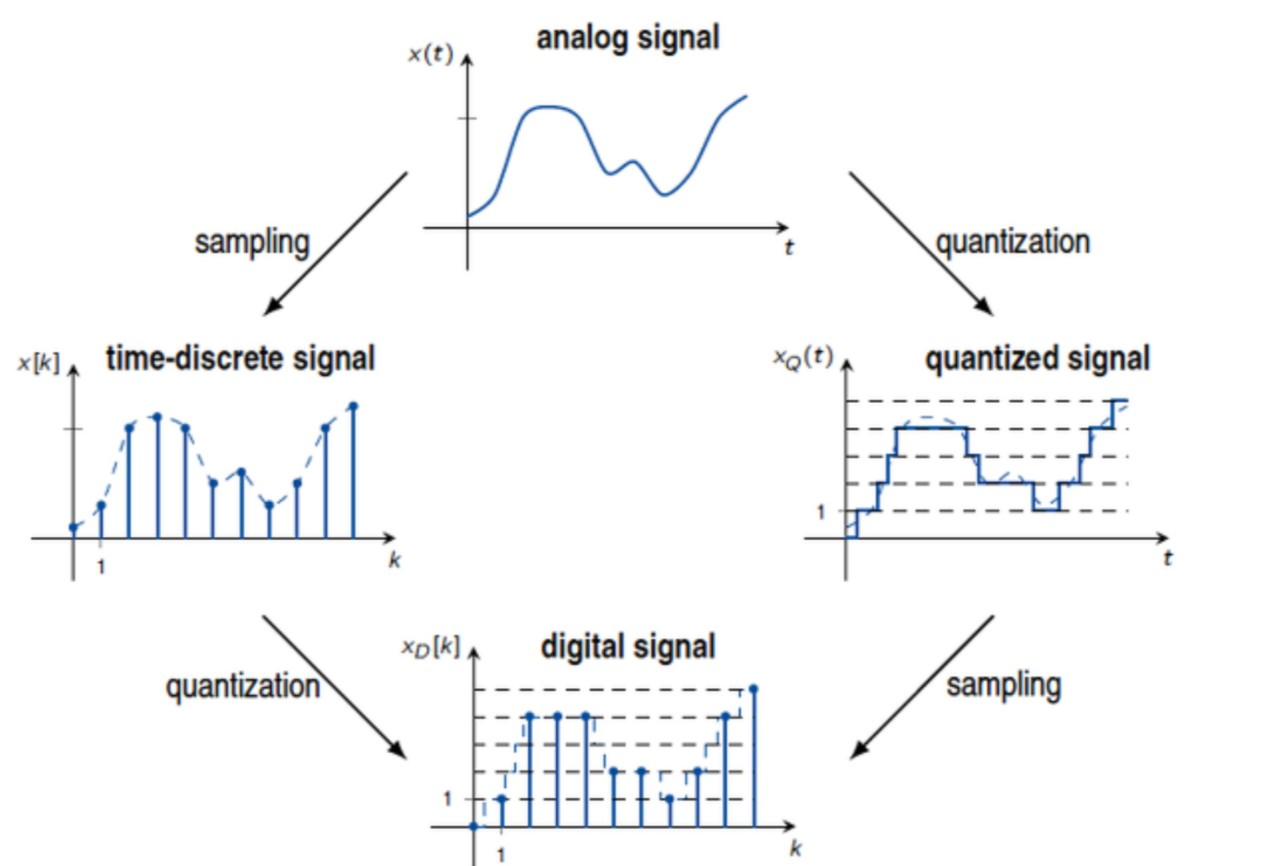
\includegraphics[width=0.8\textwidth]{figures/6-15.jpg}
    \caption{Deux méthodes de conversion de signaux analogiques en signaux numériques. Image de Dan Boschen.}
    \label{fig:communication2}
\end{figure}
\textbf{Quantification}
La quantification est la conversion d'une quantité physique continue (par exemple la tension) en un nombre numérique (bits). Cela implique une quantification, qui introduit une erreur de quantification (d'arrondi). La valeur quantifiée est donnée par l'équation suivante :
\begin{equation}
            Q=\frac{E_{r}}{2^{M}}=\frac{V_{max}-V_{max}}{2^{M}}
\end{equation}
Où $ E_{r} $ est la plage de la variable physique, M est le nombre de bits et V est la variable physique.
\begin{figure}[H] % H force l'affichage ici
    \centering
    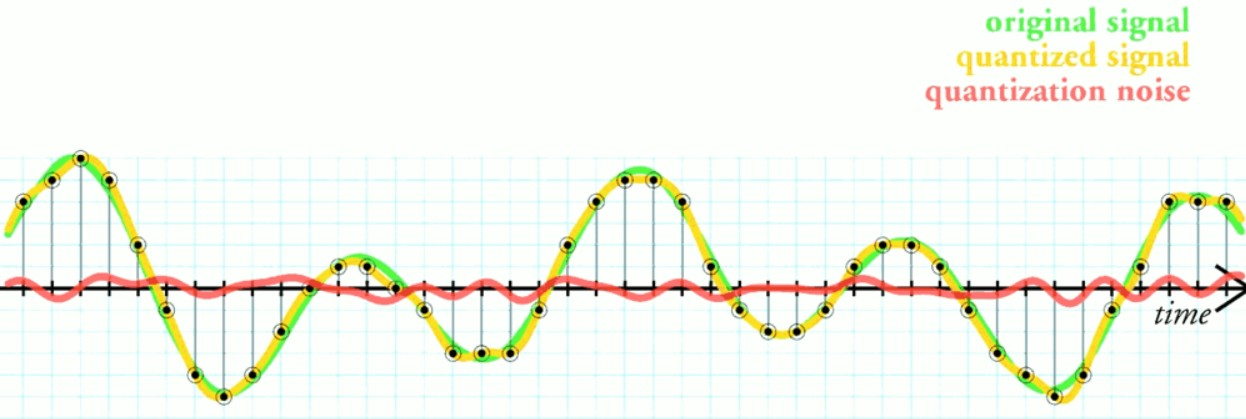
\includegraphics[width=0.8\textwidth]{figures/6-16.jpg}
    \caption{Quantification}
    \label{fig:communication2}
\end{figure}
La manière la plus simple de quantifier un signal consiste à choisir la valeur d'amplitude numérique la plus proche de l'amplitude analogique d'origine. Cet exemple montre le signal analogique d'origine (vert), le signal quantifié (points noirs), le signal reconstruit à partir du signal quantifié (jaune) et la différence entre le signal d'origine et le signal reconstruit (rouge). La différence entre le signal d'origine et le signal reconstruit est l'erreur de quantification et, dans ce schéma de quantification simple, est une fonction déterministe du signal d'entrée. Image de Gregory Maxwell.
Un exemple illustratif : disons que nous avons des mesures de température allant de \(-100^\circ C\) à \(+100^\circ C\).  
Si nous les codons avec seulement 3 bits, cela définit 8 niveaux.  
Le pas de quantification est donné par :
\[
\Delta T = \frac{200^\circ C}{8} = 25^\circ C
\]
\noindent Ce qui signifie :
\begin{itemize}
    \item Toute température comprise entre \(-100^\circ C\) et \(-75^\circ C\) est codée \(000\).
    \item Toute température comprise entre \(-75^\circ C\) et \(-50^\circ C\) est codée \(001\).
    \item \(\dots\)
    \item Toute température comprise entre \(+75^\circ C\) et \(+100^\circ C\) est codée \(111\).
\end{itemize}
Il est évident que nous avons besoin de plus de bits, car \( 25^\circ C \) n'est pas une résolution acceptable.  
Les résolutions typiques sont de 8 à 16 bits pour la plupart des mesures physiques – plus est possible.
\textbf{Échantillonnage}
Les signaux analogiques sont continus dans le temps. Pour les discrétiser, il faut les échantillonner à certains instants discrets. La fréquence d'échantillonnage est la fréquence à laquelle on prélève des échantillons du signal continu. Par exemple, dans Ariane 5, tous les capteurs fonctionnels sont échantillonnés par l'OBC à 4 Hz (toutes les 250 ms).
\begin{figure}[H] % H force l'affichage ici
    \centering
    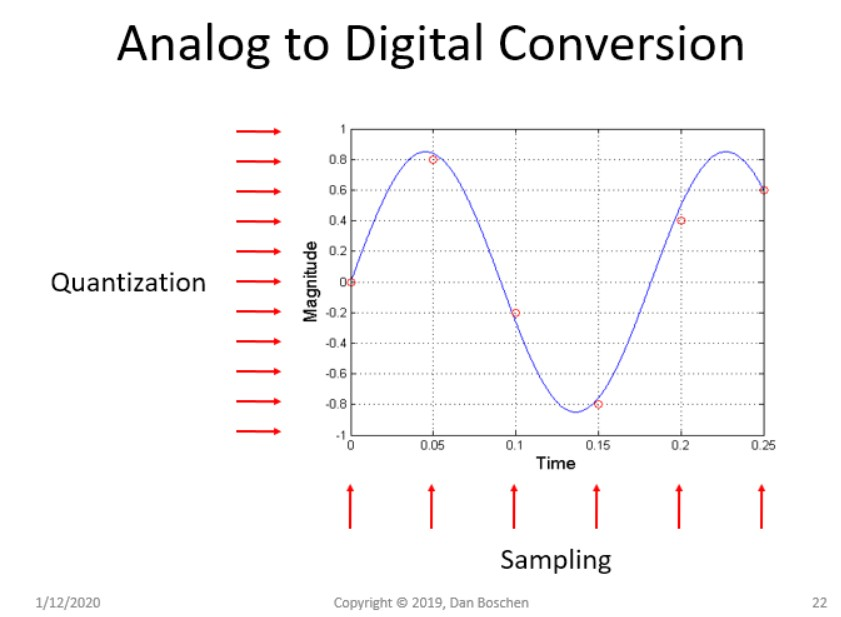
\includegraphics[width=0.8\textwidth]{figures/6-17.jpg}
        \caption{Échantillonnage}
    \label{fig:communication2}
\end{figure}
Les différences entre l'échantillonnage et la quantification sont:
\begin{itemize}
    \item Dans l'échantillonnage, \textbf{l'axe du temps} est discrétisé, tandis que dans la quantification, c'est \textbf{l'axe des y} (ou l'amplitude) qui est discrétisé.
    \item Dans le processus d'échantillonnage, \textbf{une seule valeur d'amplitude} est sélectionnée dans un intervalle de temps pour la représenter, tandis que dans la quantification, les valeurs représentant les intervalles de temps sont \textbf{arrondies} pour créer un ensemble fini de valeurs d'amplitude possibles.
    \item L'échantillonnage est effectué \textbf{avant} le processus de quantification.
\end{itemize}
\textbf{Aliasing}
À quelle fréquence devons-nous échantillonner ? Cela dépend de la rapidité avec laquelle le signal change (sa bande passante). Si nous n'échantillonnons pas assez vite, notre échantillon risque de ne pas être représentatif de la réalité.
Par exemple, deux signaux sinusoïdaux ayant des fréquences très différentes peuvent sembler identiques lorsqu’ils sont échantillonnés à basse fréquence.
\begin{figure}[H] % H force l'affichage ici
    \centering
    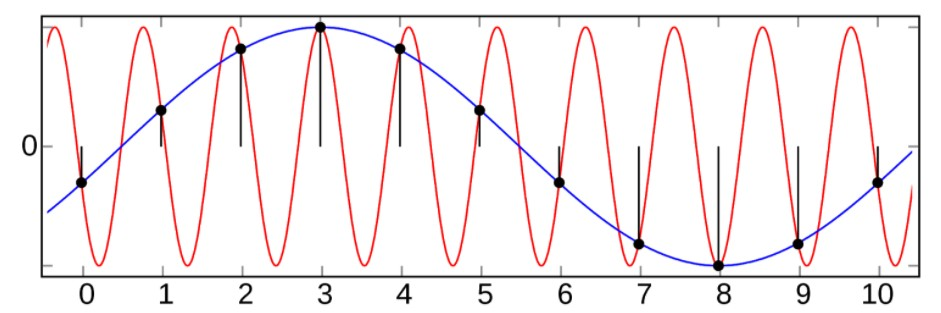
\includegraphics[width=0.8\textwidth]{figures/6-18.jpg}
    \caption{Graphique montrant l'aliasing d'une onde sinusoïdale f=0,9 par une onde sinusoïdale f=0,1 par échantillonnage à une période de T=1,0. CC BY-SA 3.0. Image de Mox Fyre.}
    \label{fig:communication2}
\end{figure}
Pour contrer l'aliasing, nous suivons le \textbf{théorème de Nyquist}, qui stipule que nous devons échantillonner au moins à :
\[
f_s = 2B
\]
où \( B \) est la bande passante.
\medskip
\noindent \textbf{Théorème de Nyquist}  
Le théorème d'échantillonnage de Nyquist-Shannon stipule :
\begin{quote}
    « Si une fonction \( x(t) \) ne contient aucune fréquence supérieure à \( B \) hertz, elle est complètement déterminée en donnant ses ordonnées à une série de points espacés de \( \frac{1}{2B} \) secondes. »
\end{quote}
Autrement dit, nous devons échantillonner au moins à :
\[
f_s = 2B
\]
(en pratique : \( f_s = 2.2B \)) où \( B \) est la limite de bande pour garantir une reconstruction parfaite du signal continu d'origine.  
Les scientifiques et les ingénieurs utilisent ce théorème pour décider de la fréquence d'échantillonnage d'un phénomène.  
Si le sujet scientifique qui nous intéresse se produit à \( B \) hertz, alors la charge utile doit échantillonner à \( 2B \) hertz.  
Si le mode dynamique d'attitude se produit à \( B \) hertz, alors l'IMU doit échantillonner à \( 2B \) hertz.
Si \( f_s - B > B \), nous pouvons alors appliquer un filtre passe-bas en \( B \) et reconstruire parfaitement le signal d'origine.
Si \( f_s - B < B \), il y a alors chevauchement (\textit{aliasing}) et nous ne pouvons pas reconstruire le signal.
\begin{figure}[H] % H force l'affichage ici
    \centering
    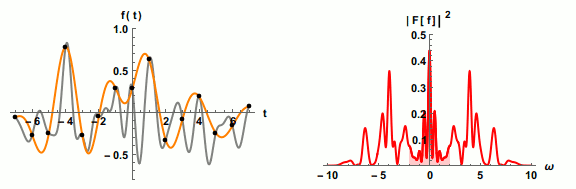
\includegraphics[width=0.8\textwidth]{figures/Nyquist_sampling.png}
    \caption{L'image de gauche montre une fonction (en gris/noir) échantillonnée et reconstruite (en doré) à des densités d'échantillonnage en constante augmentation, tandis que l'image de droite montre le spectre de fréquence de la fonction gris/noir, qui ne change pas. La fréquence la plus élevée du spectre est la moitié de la largeur du spectre entier. La largeur de l'ombrage rose en constante augmentation est égale à la fréquence d'échantillonnage. Lorsqu'elle englobe l'ensemble du spectre de fréquence, elle est deux fois plus grande que la fréquence la plus élevée, et c'est alors que la forme d'onde reconstruite correspond à celle échantillonnée. Image de Jacopo Bertolotti.}
    \label{fig:communication2}
\end{figure}
\textbf{Codage}
\begin{figure}[H] % H force l'affichage ici
    \centering
    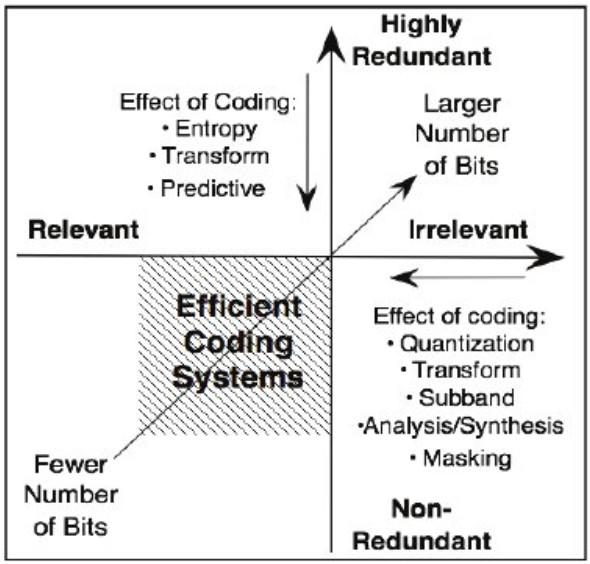
\includegraphics[width=0.8\textwidth]{figures/6-20.jpg}
    \caption{Réduction de la redondance et de la non-pertinence dans les schémas de codage. Kinsner, Witold. « L'entropie est-elle adaptée pour caractériser les données et les signaux en informatique cognitive ? » International Journal of Cognitive Informatics and Natural Intelligence (IJCINI) 1.2 (2007) : 34-57.}
    \label{fig:communication2}
\end{figure}
Le \textbf{codage source} et le \textbf{codage canal} sont deux types de codes différents utilisés dans les systèmes de communication numérique.  
Ils ont des objectifs \textbf{orthogonaux} :
\begin{itemize}
    \item L'objectif du \textbf{codage source} est la \textbf{compression des données} (diminution du débit de données).
    \item L'objectif du \textbf{codage de canal} est la \textbf{détection et correction des erreurs} (en augmentant le débit de données).
\end{itemize}
\begin{figure}[H] % H force l'affichage ici
    \centering
    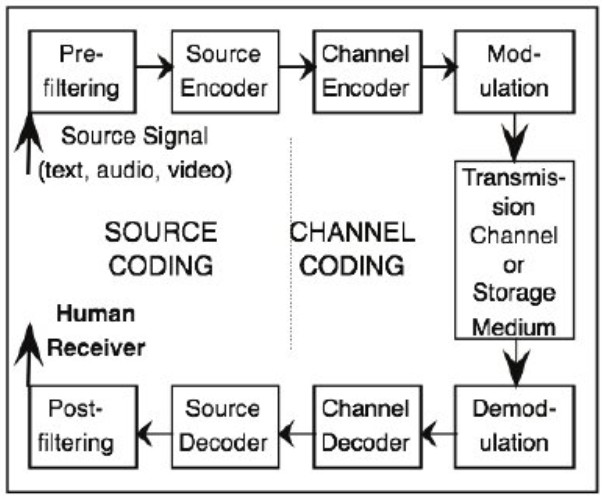
\includegraphics[width=0.8\textwidth]{figures/6-21.jpg}
    \caption{Codage conjoint source-canal-multimédia. Kinsner, Witold. « L'entropie est-elle adaptée pour caractériser les données et les signaux en informatique cognitive ? » Revue internationale d'informatique cognitive et d'intelligence naturelle (IJCINI) 1.2 (2007) : 34-57.}
    \label{fig:communication2}
\end{figure}
Le \textbf{codage source} vise à coder les données de manière plus efficace pour représenter l'information.  
Ce processus permet de \textbf{réduire la taille des données}.  
\textbf{Types de signaux et codage source} :
\begin{itemize}
    \item \textbf{Signaux analogiques} : Encodage des données analogiques dans un format binaire.
    \item \textbf{Signaux numériques} : Réduction de la taille des données sources numériques.
\end{itemize}
\textbf{Compression des données} :  
Il existe deux types de compression :
\begin{itemize}
    \item \textbf{Compression sans perte} :
    \begin{itemize}
        \item Permet une \textbf{reconstruction parfaite} du signal d'origine.
        \item Utilisée lorsque l'intégrité des données est essentielle.
        \item Ne permet qu'une \textbf{compression modérée} (ex. : 2:1 à 3:1) pour les images naturelles.
        \item Préconisée par de nombreux scientifiques dans les missions satellites.
        \item Exemples : fichiers \texttt{ZIP} et \texttt{PNG}.
    \end{itemize}
    \item \textbf{Compression avec perte} :
    \begin{itemize}
        \item Réduit davantage la taille des données en supprimant certaines informations.
        \item Exemples : formats \texttt{JPEG}, \texttt{MP3}, \texttt{MPEG}.
    \end{itemize}
\end{itemize}
\begin{figure}[H] % H force l'affichage ici
    \centering
    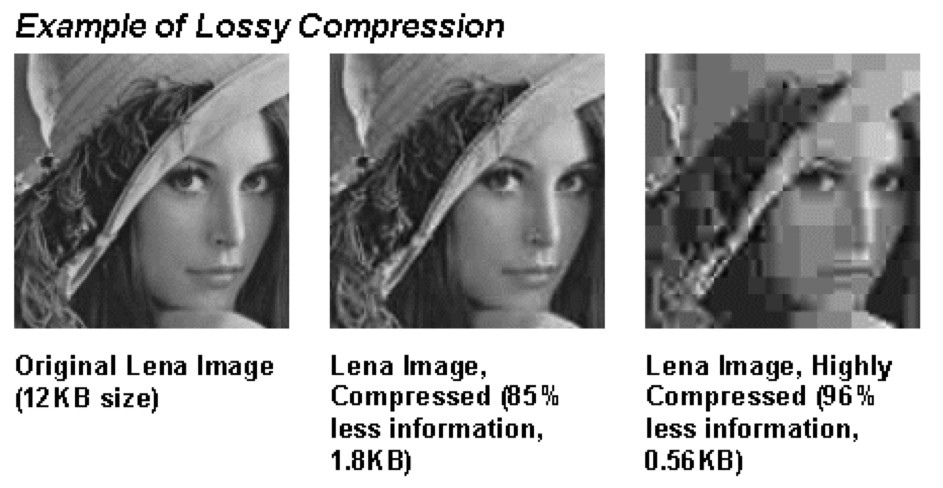
\includegraphics[width=0.8\textwidth]{figures/6-22.jpg}
    \caption{Exemple de compression avec perte. Image de Tyler Brown via WordPress.}
    \label{fig:communication2}
\end{figure}
Dans la compression avec perte, certaines informations sont perdues et une reconstruction parfaite n'est pas possible, mais en général, une réduction beaucoup plus importante du débit binaire est obtenue. Elle est utilisée lorsque la réduction du débit binaire est très importante et que l'intégrité n'est pas critique. Le codage source avec perte peut atteindre une compression beaucoup plus importante (par exemple 20:1 – 40:1) pour les images naturelles. Les exemples incluent les fichiers jpg (images) et mp3 (audio).
\begin{figure}[H] % H force l'affichage ici
    \centering
    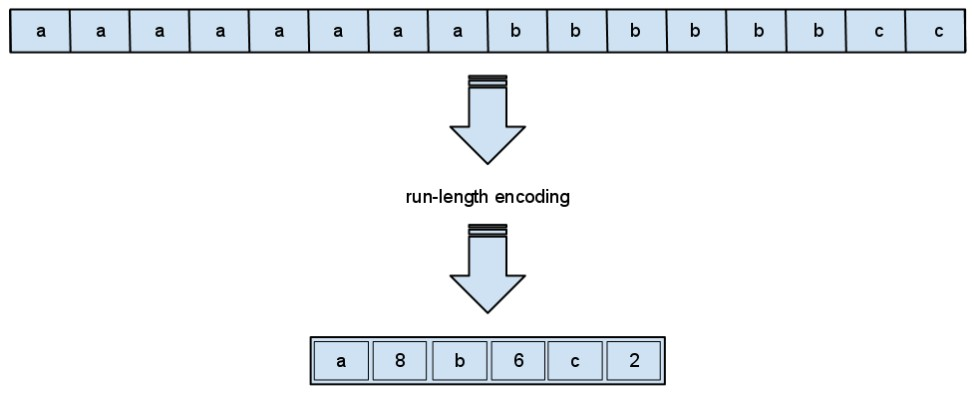
\includegraphics[width=0.8\textwidth]{figures/6-23.jpg}
    \caption{Exemple de codage de longueur d'exécution avec données originales et représentation compressée. Image du professeur GR Sinha.}
    \label{fig:communication2}
\end{figure}
Les méthodes de \textbf{compression sans perte} exploitent généralement la structure de l'information.  
Un exemple d'algorithme de compression sans perte est le \textbf{codage de longueur d'exécution} (\textit{Run-Length Encoding}, RLE). Ce type de codage est particulièrement avantageux lorsque les données contiennent des séquences répétées de la même valeur, apparaissant dans de nombreux éléments de données consécutifs.  
Dans ce cas :
\begin{itemize}
    \item Il existe des \textbf{chaînes relativement longues} de 0 ou de 1 (changements peu fréquents).
    \item Certaines \textbf{combinaisons de bits sont plus probables} que d'autres.
\end{itemize}
Dans le codage RLE, les séries de données sont stockées sous la forme d'une \textbf{valeur unique suivie du nombre de répétitions}, plutôt que d'enregistrer la série d'origine.  
\medskip
\textbf{Exemple :}  
\[
[1,0,0,0,0,0,0,0,0,0,0,1,1,\dots] \rightarrow [1,10,2]
\]
Notez que cela n'est utile que s'il existe de nombreuses longues séries de données (par exemple, de simples images en noir et blanc avec principalement du blanc).
Un autre type de compression sans perte est le codage Huffman, où si certains symboles sont plus probables que d'autres, nous pouvons utiliser moins de bits pour coder les combinaisons les plus probables. Cela entraînera des réductions du débit binaire sans perte d'informations.
\begin{figure}[H] % H force l'affichage ici
    \centering
    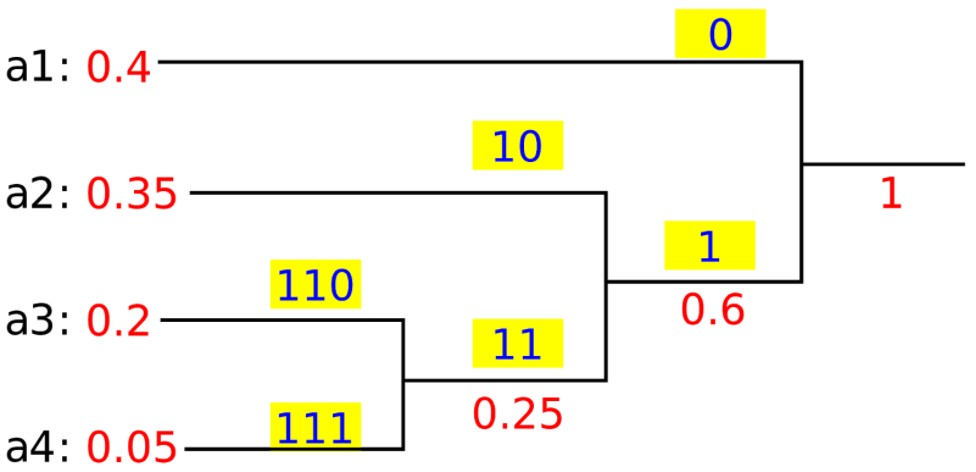
\includegraphics[width=0.8\textwidth]{figures/6-24.jpg}
    \caption{Une source génère 4 symboles différents}
    \label{fig:communication2}
\end{figure}
Le code Huffman final est présenté dans le tableau suivant :
\begin{center}
    \begin{tabular}{|c|c|}
        \hline
        \textbf{Symbole} & \textbf{Code} \\
        \hline
        $a_1$ & 1 \\
        $a_2$ & 10 \\
        $a_3$ & 110 \\
        $a_4$ & 111 \\
        \hline
    \end{tabular}
\end{center}
La manière standard de représenter un signal constitué de 4 symboles est d'utiliser 2 bits/symbole, mais l'entropie de la source est de 1,74 bits/symbole. Si ce code de Huffman est utilisé pour représenter le signal, alors la longueur moyenne est abaissée à 1,85 bits/symbole ; on est encore loin de la limite théorique car les probabilités des symboles sont différentes des puissances négatives de deux.
L'algorithme de \textbf{codage de Huffman} est le suivant :
\begin{itemize}
    \item Attribuez \textbf{0} au symbole le plus probable, les autres commencent par \textbf{1}.
    \item Attribuez \textbf{10} au symbole le plus probable parmi les restants, les autres commencent par \textbf{11}.
    \item Continuez ce processus récursivement jusqu'à ce que tous les symboles soient codés.
\end{itemize}
\textbf{Codes préfixes :} comment savoir quand commence un symbole s'il est de longueur variable ?  
Les codes préfixes (comme Huffman) ne nécessitent aucun marqueur malgré leur longueur variable, car ils sont conçus de manière à éviter toute confusion possible.
\textbf{Codage des canaux :}  
Le codage des canaux a pour but de garantir que les données reçues sont identiques à celles envoyées.  
\textit{« Les liaisons sans fil souffrent d’interférences et d’évanouissements qui provoquent des erreurs. Pour y remédier, l’émetteur ajoute des informations supplémentaires avant l’envoi des données. Ensuite, du côté du récepteur, des codes complexes nécessitant des algorithmes sophistiqués décodent ces informations et récupèrent les données d’origine. »}  
La détection et la correction des erreurs reposent sur une idée clé : ajouter des bits de redondance de manière stratégique pour éviter les erreurs.
\textbf{Comment détecter une erreur ?}  
Imaginons que nous ajoutions un bit de parité à la fin de chaque bit $N$ de sorte que la somme de tous les bits, y compris le bit de parité, soit toujours égale à 0. Nous pouvons alors détecter une erreur :
\begin{align*}
01010101 &\quad \text{→ somme = 0, OK aucune erreur. (ou il pourrait y avoir 2 erreurs !)} \\
11101100 &\quad \text{→ somme = 1, NOK. Il y a une erreur (mais je ne peux pas la corriger)}
\end{align*}
\textbf{Comment corriger une erreur ?}  
Imaginons que nous transmettions simplement chaque bit 3 fois. Il y a alors deux symboles possibles : 000 et 111. Nous disons que le code a une distance de 3 car 3 bits doivent changer pour transformer un symbole valide en un autre.
\begin{align*}
100, 010, 001 &\quad \text{→ corrigé à 000} \\
110, 101, 011 &\quad \text{→ corrigé à 111}
\end{align*}
\begin{figure}[H] % H force l'affichage ici
    \centering
    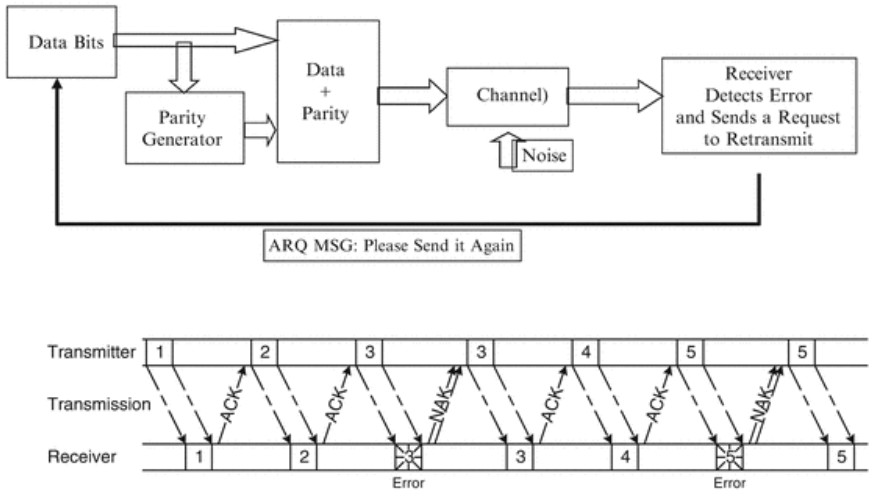
\includegraphics[width=0.8\textwidth]{figures/6-25.jpg}
    \caption{Boucle de codage de canal où la parité est non seulement ajoutée mais où le récepteur vérifie si une erreur a été détectée, un message de demande de répétition automatique (ARQ) est envoyé. Image de Springer Link.}
    \label{fig:communication2}
\end{figure}
Si nous détectons une erreur, nous pouvons demander une retransmission. On parle alors parfois de correction d'erreur en amont. Cela s'oppose à la correction d'erreur en aval (FEC) dans laquelle la correction d'erreur est intégrée à la transmission. 
Propriétés des codes FEC :
\begin{itemize}
    \item \textbf{Distance} : nombre minimum de bits nécessaires pour effectuer une transformation entre deux symboles valides.
    \item \textbf{Nombre d'erreurs détectées/corrigées}.
    \item \textbf{Taux} : Nombre de bits de données / Nombre total de bits  
          \( \rho = \frac{n - r}{n} \)
    \item \textbf{Gain de code} : Gain en dB dans l'équation de budget de liaison pour un BER (taux d'erreur binaire) égal.
\end{itemize}
Deux principaux types de codes correcteurs d’erreurs :
\begin{itemize}
    \item \textbf{Codes de bloc} :
          \begin{itemize}
              \item Codes de Hamming
              \item Reed-Salomon
          \end{itemize}
    \item \textbf{Codes convolutifs} :
          \begin{itemize}
              \item Viterbi
          \end{itemize}
\end{itemize}
Les codes de Hamming sont une famille de codes correcteurs d'erreurs linéaires. Le code de Hamming est le code Hadamard raccourci. Les codes de Hamming peuvent détecter des erreurs allant jusqu'à deux bits ou corriger des erreurs d'un bit sans détecter d'erreurs non corrigées. En revanche, le code de parité simple ne peut pas corriger les erreurs et ne peut détecter qu'un nombre impair de bits erronés. Les codes de Hamming sont des \textbf{codes parfaits}, c'est-à-dire qu'ils atteignent le taux le plus élevé possible pour des codes avec leur longueur de bloc et leur distance minimale de trois.
\begin{figure}[H] % H force l'affichage ici
    \centering
    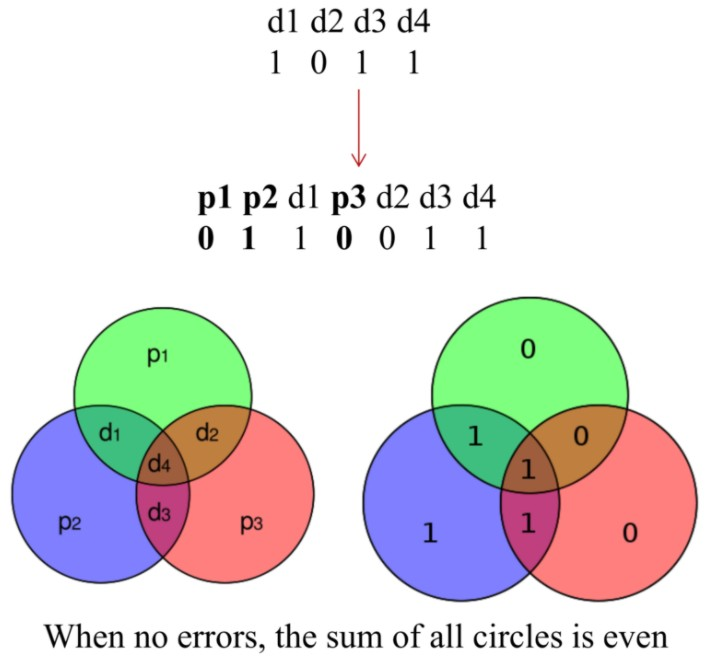
\includegraphics[width=0.8\textwidth]{figures/6-26.jpg}
    \caption{Le code de Hamming(7,4) (avec r = 3). Représentation graphique des quatre bits de données et des trois bits de parité et des bits de parité qui s'appliquent à quels bits de données. CC BY-SA 3.0. Image de C. Burnett.}
    \label{fig:communication2}
\end{figure}
Tous les codes de Hamming ont une distance de 3, peuvent détecter 2 erreurs et en corriger 1.  
Les longueurs des messages des codes de Hamming sont exprimées en $(2^r -1 , 2^r - r - 1)$ : (bits totaux, bits de données). Par exemple :
\begin{itemize}
    \item \textbf{Hamming(3,1)} est un message avec triple répétition.
    \item \textbf{Hamming(7,4)} est un message qui ajoute 3 bits de redondance à chaque 4 bits de données.
\end{itemize}
Le taux d'un code de bloc est défini comme le rapport entre la longueur de son message et la longueur de son bloc.  
Pour ce code de bloc, le taux est de $ \frac{4}{7} $.
Les bits de parité sont ajoutés aux positions $ 1, 2, 4, 8, \dots $. Les autres sont des bits de données.  
Chaque bit de parité couvre un sous-ensemble différent de bits :  
Le bit de parité 1 couvre toutes les positions de bits dont le bit le moins significatif est défini (1, 3, 5, …).
\begin{figure}[H] % H force l'affichage ici
    \centering
    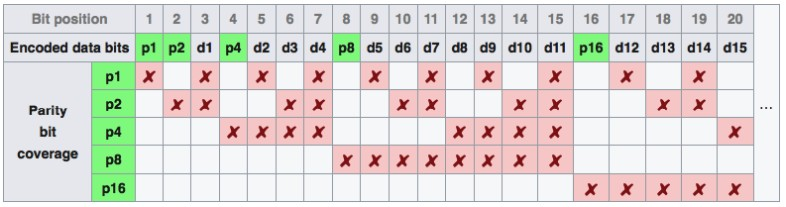
\includegraphics[width=0.8\textwidth]{figures/6-27.jpg}
    \caption{L'algorithme général suivant génère un code de correction d'erreur unique (SEC) pour n'importe quel nombre de bits. Seuls 20 bits codés (5 de parité, 15 de données) sont représentés, mais le modèle se poursuit indéfiniment. L'élément clé des codes de Hamming qui peut être vu à partir d'une inspection visuelle est que chaque bit donné est inclus dans un ensemble unique de bits de parité. Pour vérifier les erreurs, vérifiez tous les bits de parité. Image par Artillar. }
    \label{fig:communication2}
\end{figure}
Intuitivement, 1 erreur peut être corrigée grâce à la distance de 3 entre les symboles valides. Comme chaque bit est affecté à un ensemble unique de bits de parité, nous pouvons identifier quel bit est erroné en identifiant le bit pour lequel tous les bits de parité sont erronés d2. La position du bit erroné est égale à la somme des positions de tous les bits de parité erronés : 1(p1) + 4(p3) = 5 (d2).
\begin{figure}[H] % H force l'affichage ici
    \centering
    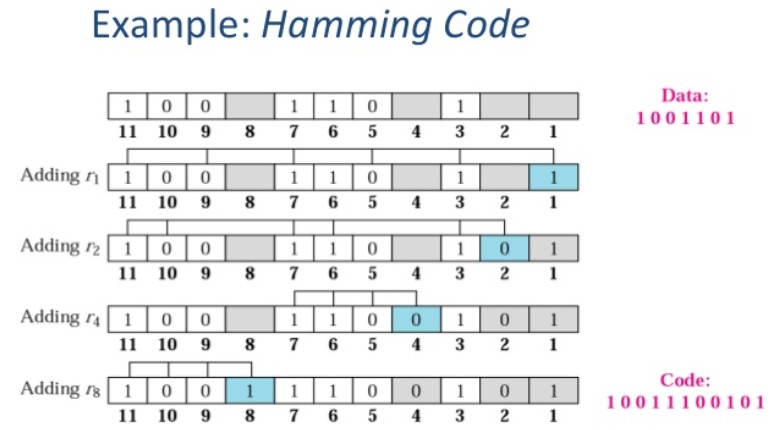
\includegraphics[width=0.8\textwidth]{figures/6-28.jpg}
    \caption{Exemple de code de Hamming. CC-BY SA 4. Image par Artillar.}
    \label{fig:communication2}
\end{figure}
Un autre algorithme de codage de canal est appelé \textbf{code de correction d'erreurs Reed-Solomon}.  
Contrairement aux algorithmes basés sur les bits, l'algorithme Reed-Solomon opère sur des \textit{symboles}, généralement constitués de blocs de 8 bits.  

Ce type de codage est particulièrement efficace pour la correction des \textit{erreurs en rafale}, car plusieurs bits erronés peuvent être considérés comme un seul symbole erroné.  
Le code Reed-Solomon convertit $k$ symboles de données en $n > k$ symboles redondants à l'aide de polynômes, permettant ainsi de détecter et de corriger un certain nombre d'erreurs.
Codage Reed-Solomon pour la tolérance aux pannes. Accélérez le codage Reed-Solomon pour la tolérance aux pannes dans un système de type RAID par Shuai Yuan.
\begin{figure}[H] % H force l'affichage ici
    \centering
    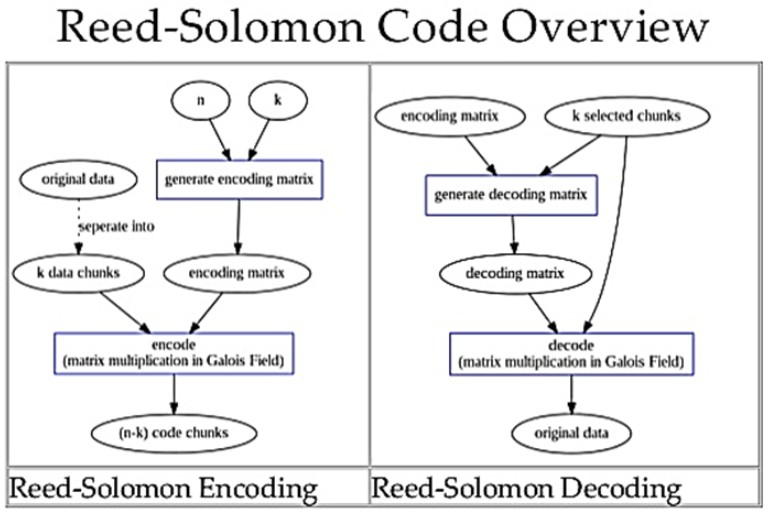
\includegraphics[width=0.8\textwidth]{figures/6-29.jpg}
    
    \caption{Codage Reed-Solomon pour la tolérance aux pannes. Accélérez le codage Reed-Solomon pour la tolérance aux pannes dans un système de type RAID par Shuai Yuan.}
    \label{fig:communication2}
\end{figure}
\textbf{Codage : deux étapes}
\begin{itemize}
    \item Interpréter le message $x = [x_1, x_2, \dots, x_k]$ comme les coefficients d'un polynôme de degré $k - 1$ :
    \[
    p_x(a) = \sum_{i=1}^{k} x_i a^{i-1}
    \]
    
    \item Évaluer le polynôme en $n$ points différents :
    \[
    C(x) = [p_x(a_1), p_x(a_2), \dots, p_x(a_n)]
    \]
\end{itemize}
\textbf{Décodage :} Basé sur la régression (trouver un polynôme qui passe par les $n$ points).
Par exemple, Reed-Solomon (255,223) ajoute 32 symboles redondants pour 223 symboles de données. Il peut détecter 32 erreurs et en corriger 16. Read-Solomon est utilisé de manière exhaustive dans l'espace, notamment en concaténation avec des codes convolutifs (par exemple Voyager, Meteosat, Timed).
\begin{figure}[H] % H force l'affichage ici
    \centering
    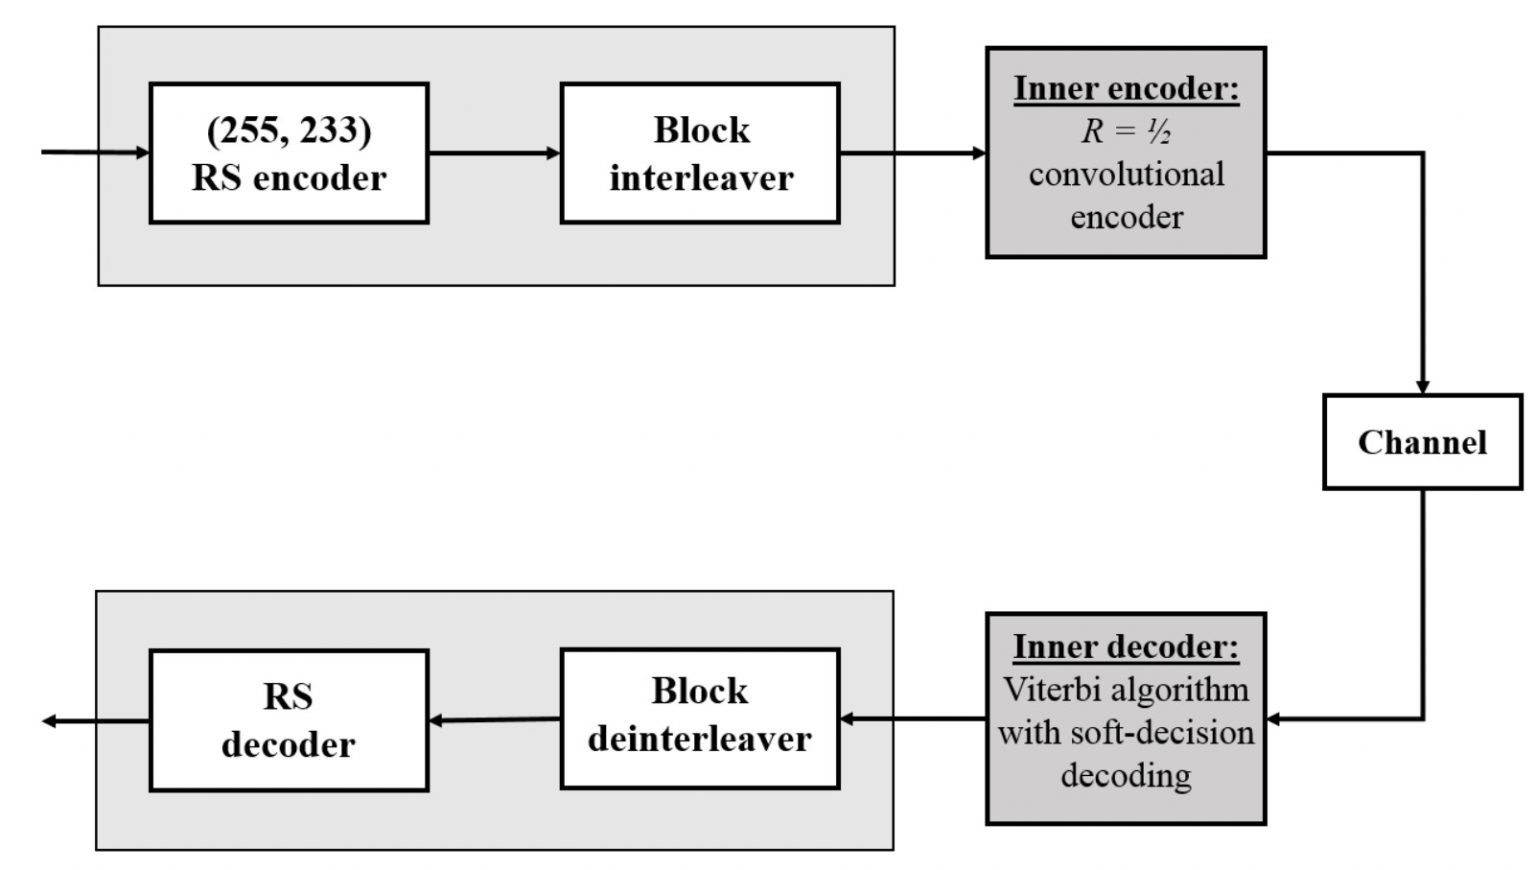
\includegraphics[width=0.8\textwidth]{figures/6-30.jpg}
    \caption{Système de codage concaténé en espace profond. Notation : RS(255, 223) + CC (« longueur de contrainte » = 7, taux de codage = 1/2). CC BY-SA 4.0. Image de Kirlf.}
    \label{fig:communication2}
\end{figure}
\begin{figure}[H] % H force l'affichage ici
    \centering
    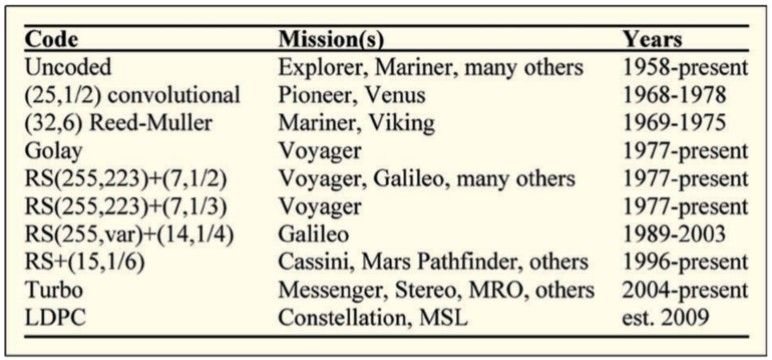
\includegraphics[width=0.8\textwidth]{figures/6-31.jpg}
    \caption{Codes Used by NASA Missions Andrews, Kenneth S., et al. “The development of turbo and LDPC codes for deep-space applications.” Proceedings of the IEEE 95.11 (2007): 2142-2156. Image by IEEE Explore.}
    \label{fig:communication2}
\end{figure}
\textbf{Modulations}
\textbf{Lectures suggérées :} 
\href{https://deepspace.jpl.nasa.gov/dsndocs/810-005/208/208B.pdf}{\textit{Système de télémétrie DSN, décodage des données}}
Les informations entre le satellite et la station terrestre sont transmises en modifiant certaines propriétés (amplitude, fréquence ou phase) d'un signal porteur haute fréquence $c(t)$ de manière à coder les informations dans le message $m(t)$.  
C'est ce qu'on appelle la \textbf{modulation}. Il existe un schéma de modulation pour les signaux analogiques et numériques que nous examinerons dans cette section.
\vspace{0.5cm}
\textbf{Pourquoi avons-nous besoin de modulation ? Pourquoi ne pouvons-nous pas simplement transmettre notre train d'impulsions (bits) ?}
\begin{itemize}
    \item Ce sont des signaux de très basse fréquence.
    \item Les signaux basse fréquence nécessiteraient des antennes extrêmement grandes.
    \item Les signaux basse fréquence ont d'énormes pertes atmosphériques.
\end{itemize}
\vspace{0.5cm}
Les modulations sont basées sur la modification de la fonction sinusoïdale.  
Les trois paramètres d'une sinusoïde qui peuvent être modifiés sont :
\begin{itemize}
    \item \textbf{Amplitude}
    \item \textbf{Fréquence}
    \item \textbf{Phase}
\end{itemize}
\textbf{Modulation d'amplitude (AM)}
\begin{figure}[H] % H force l'affichage ici
    \centering
    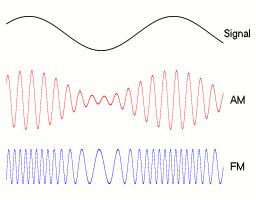
\includegraphics[width=0.8\textwidth]{figures/Amfm3-en-de-0003.jpg}
    \caption{Diagramme représentant la différence entre les ondes radio modulées en amplitude et en fréquence. CC BY-SA 2.5. Image de Berserkerus. }
    \label{fig:communication2}
\end{figure}
« La modulation d'amplitude (AM) est une technique de modulation utilisée dans les communications électroniques, le plus souvent pour transmettre des messages avec une onde porteuse radio . Dans la modulation d'amplitude, l' amplitude (intensité du signal) de l'onde porteuse varie proportionnellement à celle du signal du message » . Cet algorithme modulaire est facile à mettre en œuvre mais présente de faibles performances en matière de bruit.
\begin{figure}[H] % H force l'affichage ici
    \centering
    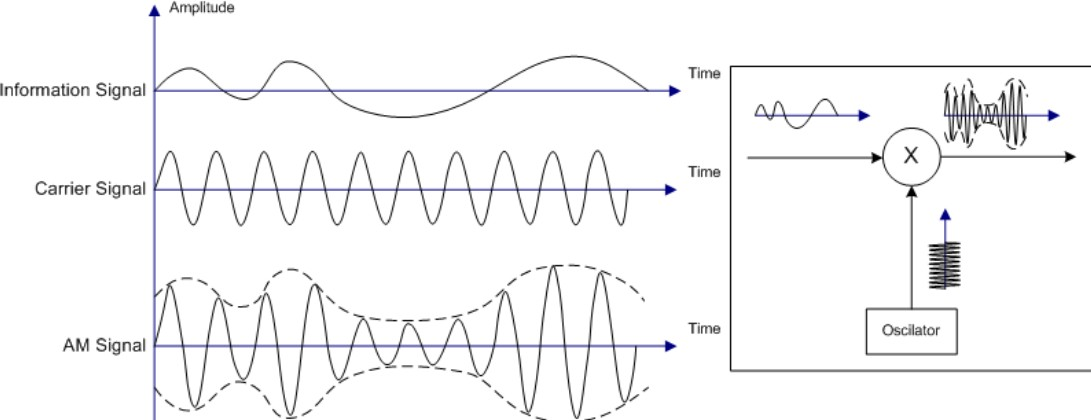
\includegraphics[width=0.8\textwidth]{figures/6-32.jpg}
    \caption{L'illustration de la modulation d'amplitude (AM) montre une comparaison entre un signal d'information, un signal porteur et un signal AM. CC BY-SA 3.0. Image par Ivan }
    \label{fig:communication2}
\end{figure}
Supposons que le signal porteur à la fréquence radio sous licence ait la forme :  
\[
c(t) = A_c \cos(\omega_c t).
\]
Le signal analogique est $m(t)$ avec une bande passante $B$, généralement $B \ll \omega_c$.  
Des exemples de signaux analogiques sont :
\begin{itemize}
    \item L'audio autour de $4$ kHz.
    \item La vidéo à $4$ MHz.
\end{itemize}
Le signal modulé en amplitude à la fréquence radio sous licence est donné par :
\[
s_{AM} (t) = A_c (1 + m(t)) \cos(\omega_c t).
\]
\begin{figure}[H] % H force l'affichage ici
    \centering
    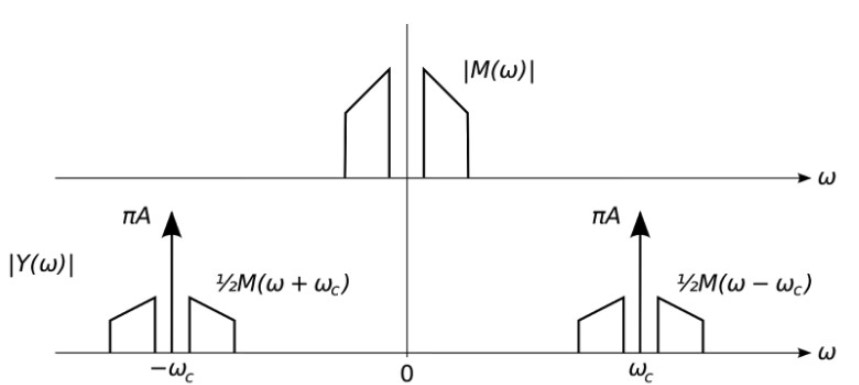
\includegraphics[width=0.8\textwidth]{figures/6-121.jpg}
  \caption{Spectres bilatéraux des signaux en bande de base et AM. CC BY-SA 3.0. Image de Splash. }
    \label{fig:communication2}
\end{figure}
\textbf{La modulation d'amplitude nécessite :}
\begin{itemize}
    \item Un oscillateur local pour générer le signal porteur haute fréquence.
    \item Un mixeur pour mélanger (multiplier) les deux signaux.
    \item Un amplificateur.
\end{itemize}
\begin{figure}[H] % H force l'affichage ici
    \centering
    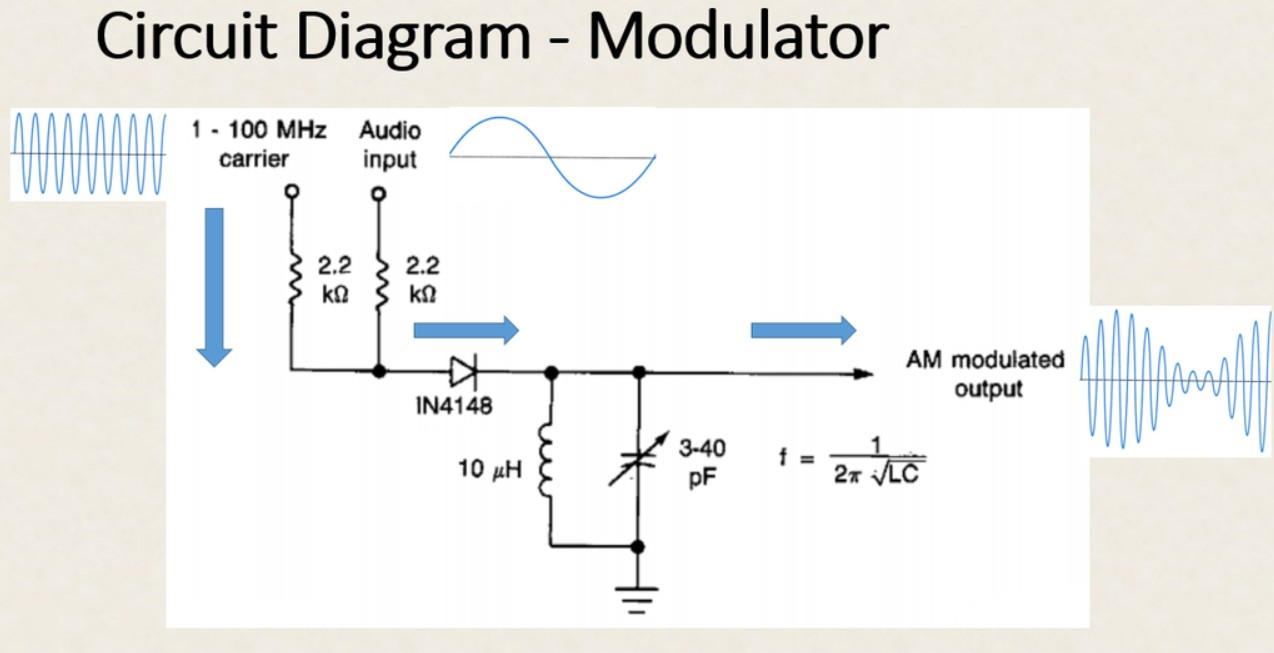
\includegraphics[width=0.8\textwidth]{figures/6-34.jpg}
    \caption{Ce modulateur à diode simple fournit d'excellents résultats lorsqu'il est utilisé pour une modulation à pourcentage élevé à de faibles niveaux de signal. Image par Instructables.}
    \label{fig:communication2}
\end{figure}
\textbf{La démodulation du signal nécessite :}
\begin{itemize}
    \item Un oscillateur local pour générer un proxy du signal porteur.
    \item Un mixeur pour multiplier.
    \item Un filtre passe-bas pour ne conserver que la partie basse fréquence du signal reçu.
    \item Une diode pour supprimer la partie DC.
\end{itemize}
\begin{figure}[H] % H force l'affichage ici
    \centering
    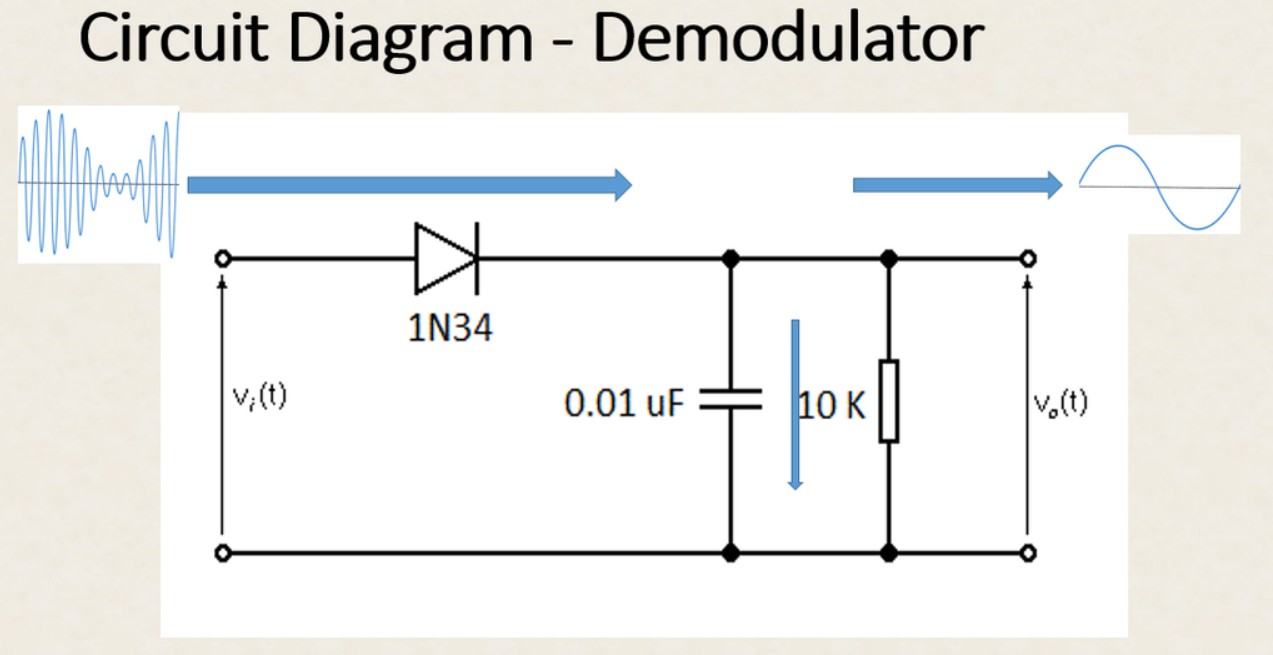
\includegraphics[width=0.8\textwidth]{figures/6-35.jpg}
    \caption{La combinaison du condensateur C et de la résistance R se comporte comme un filtre passe-bas. Le signal d'entrée contient à la fois le message d'origine et l'onde porteuse, le condensateur aidant à filtrer les ondes porteuses RF. Le condensateur se charge pendant le front montant et se décharge à travers la résistance R pendant le front descendant. Ainsi, le condensateur permet de donner une enveloppe de l'entrée en sortie. Image par Instructables.}
    \label{fig:communication2}
\end{figure}
\textbf{Modulation de fréquence (FM)}
\begin{figure}[H] % H force l'affichage ici
    \centering
    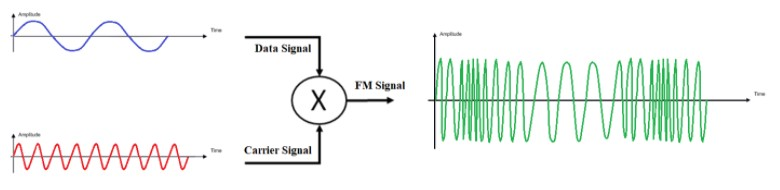
\includegraphics[width=0.8\textwidth]{figures/6-36.jpg}
    \caption{La modulation d'un signal analogique en une porteuse analogique en utilisant la modulation de fréquence (FM). CC BY-SA 4.0. Image de Michel Bakni.}
    \label{fig:communication2}
\end{figure}
« La modulation de fréquence (FM) est le codage d' informations dans une onde porteuse en faisant varier la fréquence instantanée de l'onde. Cette technologie est utilisée dans les télécommunications , la radiodiffusion , le traitement du signal et l'informatique . Dans la transmission radio, l'un des avantages de la modulation de fréquence est qu'elle présente un rapport signal/bruit plus élevé et qu'elle rejette donc mieux les interférences radioélectriques qu'un signal de modulation d'amplitude (AM) de puissance égale » 
\begin{figure}[H] % H force l'affichage ici
    \centering
    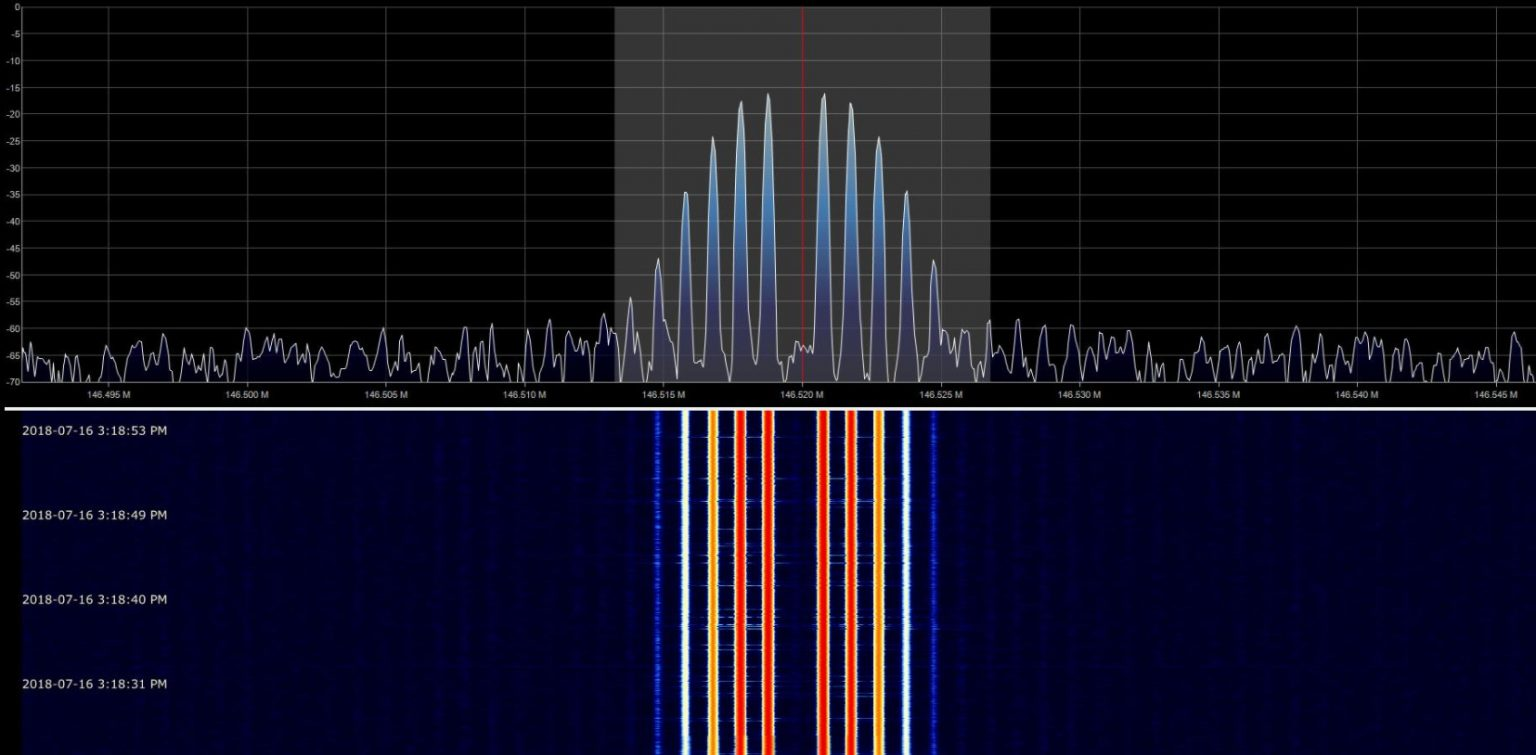
\includegraphics[width=0.8\textwidth]{figures/6-37.jpg}
    \caption{Spectre de fréquence et courbe en cascade d'une porteuse de 146,52 MHz, modulée en fréquence par une sinusoïde de 1 000 Hz. L'indice de modulation a été ajusté à environ 2,4, de sorte que la fréquence porteuse a une faible amplitude. Plusieurs bandes latérales fortes sont apparentes ; en principe, un nombre infini de bandes latérales sont produites en FM, mais les bandes latérales d'ordre supérieur sont d'une amplitude négligeable. CC BY-SA 4.0. Image de Wtshymanski.}
    \label{fig:communication2}
\end{figure}
Supposons à nouveau un signal porteur de la forme :  
\[
c(t) = A_c \cos(\omega_c t).
\]
Le signal analogique que nous essayons de convertir est de la forme $m(t)$ avec une bande passante $B$, typiquement $B \ll \omega_c$.  
Le signal modulé en fréquence prend la forme :
\[
s_{FM}(t) = A_c \cos\left( \int_0^t (\omega_c + f_{\Delta} m (\tau)) \, d\tau \right) 
= A_c \cos\left(\omega_c t + f_{\Delta} \int_0^t m (\tau) \, d\tau \right).
\]
\textbf{Caractéristiques du spectre et de la modulation FM :}
\begin{itemize}
    \item Le spectre d'un signal FM est difficile à calculer analytiquement, même pour des messages simples.
    \item La modulation et la démodulation FM sont similaires à l'AM en principe, mais nécessitent des intégrateurs et des différenciateurs.
    \item La modulation de fréquence nécessite une boucle de verrouillage de fréquence, qui peut être mise en œuvre avec des résistances, des condensateurs et des amplificateurs opérationnels, par exemple.
\end{itemize}
\textbf{Types de modulation FM :}
\begin{itemize}
    \item \textbf{Modulation FM directe} : obtenue en alimentant directement le message dans l'entrée d'un oscillateur contrôlé en tension.
    \item \textbf{Modulation FM indirecte} :
    \begin{itemize}
        \item Le signal de message est intégré pour générer un signal modulé en phase.
        \item Ce signal est utilisé pour moduler un oscillateur contrôlé par cristal.
        \item Le résultat est passé à travers un multiplicateur de fréquence pour produire un signal FM.
        \item Une FM à bande étroite est générée en premier, puis transformée en FM à large bande.
        \item Cette technique est connue sous le nom de \textbf{modulation FM indirecte}.
    \end{itemize}
\end{itemize}
\textbf{Méthodes de démodulation FM :}
\begin{itemize}
    \item Une méthode courante pour récupérer le signal d'information consiste à utiliser un \textbf{discriminateur Foster-Seeley} ou un \textbf{détecteur de rapport}.
    \item Une \textbf{boucle à verrouillage de phase (PLL)} peut être utilisée comme démodulateur FM.
    \item La \textbf{détection de pente} démodule un signal FM en utilisant un circuit accordé dont la fréquence de résonance est légèrement décalée par rapport à la porteuse.  
    \begin{itemize}
        \item Lorsque la fréquence monte et descend, le circuit accordé fournit une amplitude de réponse variable.
        \item Cette variation convertit la FM en AM.
    \end{itemize}
\end{itemize}
\begin{figure}[H] % H force l'affichage ici
    \centering
    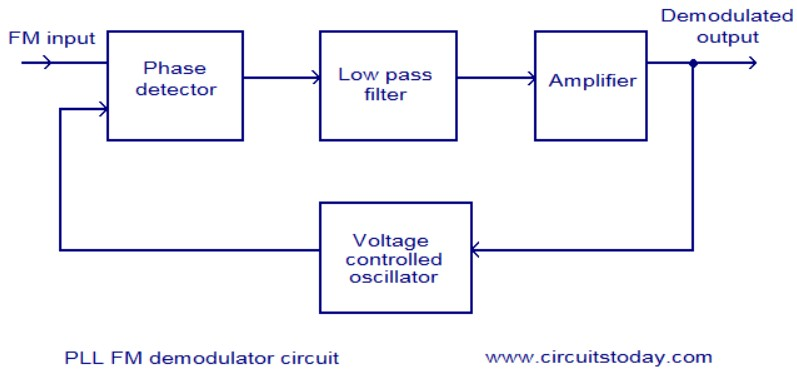
\includegraphics[width=0.8\textwidth]{figures/6-38.jpg}
    \caption{Modulateur de fréquence à boucle à verrouillage de phase (PLL FM). Le signal FM d'entrée et la sortie de l'oscillateur contrôlé en tension (VCO) sont appliqués au circuit détecteur de phase. La sortie du détecteur de phase est filtrée à l'aide d'un filtre passe-bas, de l'amplificateur, puis utilisée pour contrôler le VCO. Lorsqu'il n'y a pas de modulation de porteuse et que le signal FM d'entrée est au centre de la bande passante, la tension de ligne de réglage du VCO sera à la position centrale. Lorsqu'une déviation de la fréquence porteuse se produit (ce qui signifie qu'une modulation se produit), la fréquence du VCO suit le signal d'entrée afin de maintenir la boucle verrouillée. En conséquence, la tension de ligne de réglage du VCO varie et cette variation est proportionnelle à la modulation effectuée sur l'onde porteuse FM. La variation de tension est filtrée et amplifiée afin d'obtenir le signal démodulé. Image de Circuits Today.}
    \label{fig:communication2}
\end{figure}
\textbf{Modulation de phase}
\textbf{Modulation de phase (PM) :}
\begin{itemize}
    \item La modulation de phase (PM) est un modèle de modulation permettant de conditionner les signaux de communication en vue de leur transmission.
    \item Elle code un signal de message sous forme de variations de la phase instantanée d'une onde porteuse.
    \item La modulation de phase est l'une des deux principales formes de \textbf{modulation d'angle}, avec la modulation de fréquence (FM).
    \item La phase d'un signal porteur est modulée pour suivre le niveau de signal changeant (amplitude) du signal de message.
    \item L'amplitude de crête et la fréquence du signal porteur sont maintenues constantes, mais lorsque l'amplitude du signal de message change, la phase du signal porteur change en conséquence.
    \item La modulation de phase est largement utilisée pour transmettre des ondes radio.
    \item Elle fait partie intégrante de nombreux schémas de codage de transmission numérique, sous-tendant un large éventail de technologies, telles que :
    \begin{itemize}
        \item \textbf{Wi-Fi},
        \item \textbf{GSM},
        \item \textbf{Télévision par satellite}.
    \end{itemize}
\end{itemize}
\begin{figure}[H] % H force l'affichage ici
    \centering
    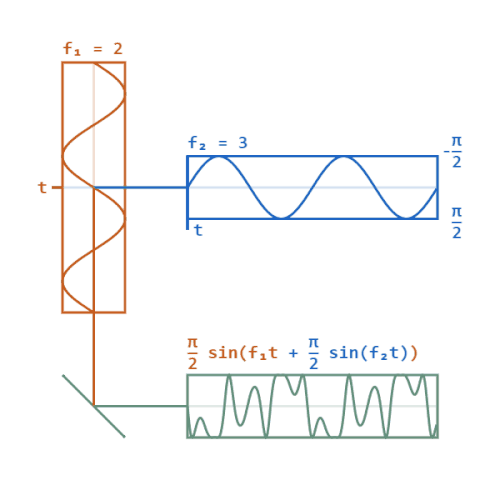
\includegraphics[width=0.8\textwidth]{figures/500px-Phase-modulation.png}
    \caption{L'onde modulante (bleue) module l'onde porteuse (rouge), ce qui donne le signal PM (vert). Image de Potasmic.}
    \label{fig:communication2}
\end{figure}
Supposons à nouveau un signal porteur de la forme :  
\[
c(t) = A_c \cos(\omega_c t + \phi_c).
\]
Le signal analogique que nous essayons de convertir est de la forme $m(t)$ avec une bande passante $B$, typiquement $B \ll \omega_c$.  
Le signal modulé en phase prend la forme :
\[
s_{PM}(t) = A_c \cos(\omega_c t + m(t) + \phi_c).
\]
\begin{figure}[H] % H force l'affichage ici
    \centering
    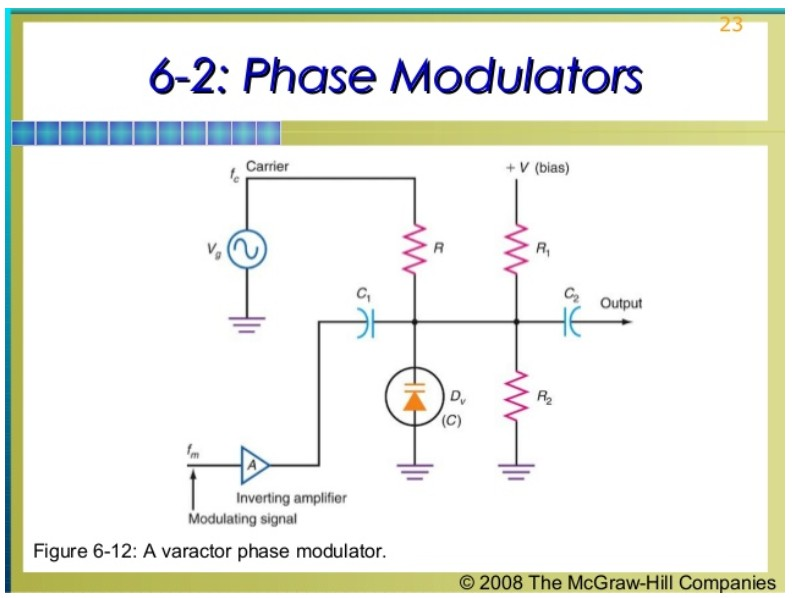
\includegraphics[width=0.8\textwidth]{figures/6-39.jpg}
    \caption{Schéma de principe du modulateur de phase. Image de McGraw-Hill Companies.}
    \label{fig:communication2}
\end{figure}
\textbf{Système de contrôle à boucle de verrouillage de phase (PLL) :}

\begin{itemize}
    \item La modulation de phase nécessite un \textbf{système de contrôle à boucle de verrouillage de phase} (PLL).
    \item Il existe plusieurs types de PLL, le plus simple étant un circuit électronique comprenant :
    \begin{itemize}
        \item Un \textbf{oscillateur à fréquence variable}.
        \item Un \textbf{détecteur de phase} dans une boucle de rétroaction.
    \end{itemize}
    \item Fonctionnement :
    \begin{itemize}
        \item L'oscillateur génère un signal périodique.
        \item Le détecteur de phase compare la phase du signal généré à celle du signal périodique d'entrée.
        \item Le détecteur ajuste l'oscillateur pour maintenir les phases correspondantes.
    \end{itemize}
\end{itemize}

\textbf{Modulation numérique :}

\begin{itemize}
    \item Contrairement à la modulation analogique, la \textbf{modulation numérique} transforme un signal binaire.
    \item Le signal porteur reste un signal analogique.
    \item La modulation numérique utilise un \textbf{nombre fini de signaux analogiques} (impulsions) pour représenter des parties d'un message numérique.
    \item Exemple :
    \begin{itemize}
        \item Le code \textbf{00} peut être représenté par : 
        \[
        A_c \cos(\omega_c t).
        \]
        \item Nous pouvons encoder un \textbf{0} comme :
        \[
        \cos(\omega_0 t),
        \]
        \item et un \textbf{1} comme :
        \[
        \cos(\omega_1 t).
        \]
    \end{itemize}
    \item Ce type de modulation est appelé \textbf{modulation par déplacement de fréquence} (FSK - Frequency Shift Keying).
    \item En \textbf{FSK binaire}, il n'y a que deux fréquences distinctes :
    \begin{itemize}
        \item \textbf{0} est transmis à la fréquence $f_0$.
        \item \textbf{1} est transmis à la fréquence $f_1$.
    \end{itemize}
    \item Nous pouvons aussi avoir des variantes comme :
    \begin{itemize}
        \item \textbf{4-FSK} : utilise 4 fréquences distinctes :
        \begin{itemize}
            \item \textbf{00} : $f_{00}$,
            \item \textbf{01} : $f_{01}$,
            \item \textbf{10} : $f_{10}$,
            \item \textbf{11} : $f_{11}$.
        \end{itemize}
        \item \textbf{8-FSK} : utilise 8 fréquences différentes, etc.
    \end{itemize}
\end{itemize}

\begin{figure}[H] % H force l'affichage ici
    \centering
    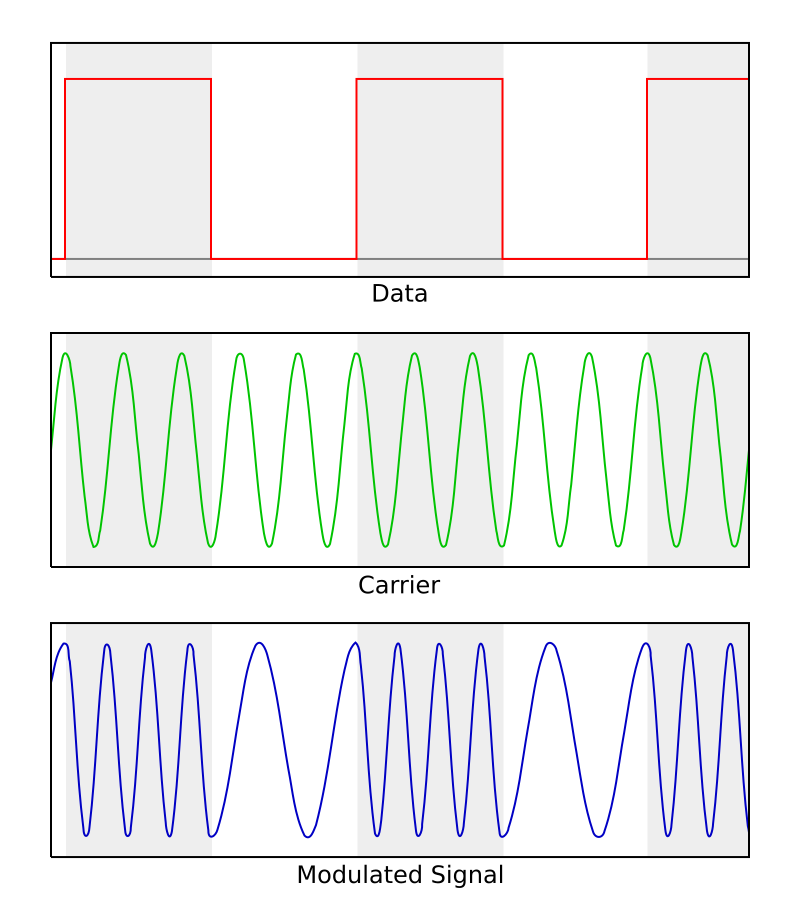
\includegraphics[width=0.8\textwidth]{figures/6-40.png}
    \caption{Exemple de FSK binaire. CC BY-SA 3.0. Image de K.Tims.}
    \label{fig:communication2}
\end{figure}
\textbf{Modulation numérique par déplacement d'amplitude (ASK) :}
\begin{itemize}
    \item Une autre méthode de modulation consiste à encoder :
    \begin{itemize}
        \item Un \textbf{0} comme :
        \[
        A_0 \cos(\omega_c t),
        \]
        \item Un \textbf{1} comme :
        \[
        A_1 \cos(\omega_c t).
        \]
    \end{itemize}
    \item Cette technique est appelée \textbf{modulation par déplacement d'amplitude} (ASK - Amplitude Shift Keying).
    \item Dans cette modulation, les \textbf{symboles correspondent à différentes amplitudes}.
    \item En \textbf{ASK binaire}, nous utilisons deux amplitudes distinctes :
    \begin{itemize}
        \item \textbf{0} est représenté par l'amplitude $A_0$,
        \item \textbf{1} est représenté par l'amplitude $A_1$.
    \end{itemize}
    \item Généralement, $A_0 = 0$.
    \item Nous pouvons également avoir des variantes comme :
    \begin{itemize}
        \item \textbf{4-ASK}, \textbf{8-ASK}, etc.
    \end{itemize}
    \item De même, pour la \textbf{4-ASK}, différentes amplitudes sont utilisées :
    \begin{itemize}
        \item \textbf{00} : $A_{00}$,
        \item \textbf{01} : $A_{01}$,
        \item \textbf{10} : $A_{10}$,
        \item \textbf{11} : $A_{11}$.
    \end{itemize}
\end{itemize}
\begin{figure}[H] % H force l'affichage ici
    \centering
    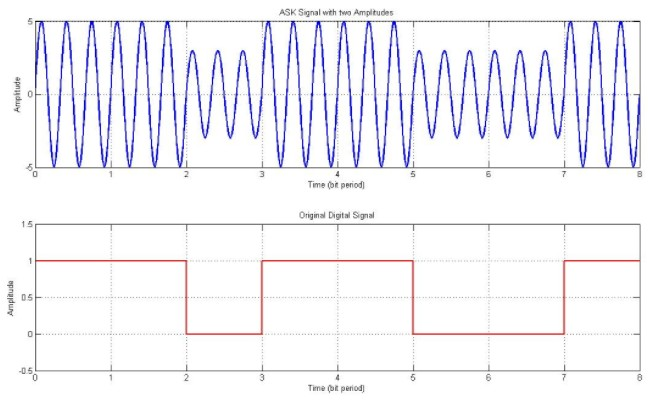
\includegraphics[width=0.8\textwidth]{figures/6-41.jpg}
    \caption{Un exemple de ASK binaire. Image de Mathworks.}
    \label{fig:communication2}
\end{figure}
\textbf{Modulation numérique par déplacement de phase (PSK) :}
\begin{itemize}
    \item Une autre méthode de modulation consiste à encoder :
    \begin{itemize}
        \item Un \textbf{0} comme :
        \[
        \cos(\omega_c t + \phi_0),
        \]
        \item Un \textbf{1} comme :
        \[
        \cos(\omega_c t + \phi_1).
        \]
    \end{itemize}
    \item Cette technique est appelée \textbf{modulation par déplacement de phase} (PSK - Phase Shift Keying).
    \item Dans cette modulation, les \textbf{symboles correspondent à différentes phases}.
    \item En \textbf{PSK binaire} (BPSK), nous utilisons deux phases distinctes :
    \begin{itemize}
        \item \textbf{0} est représenté par la phase $\phi_0$,
        \item \textbf{1} est représenté par la phase $\phi_1$.
    \end{itemize}
    \item Généralement :
    \begin{itemize}
        \item $\phi_0 = 0$,
        \item $\phi_1 = \pi$.
    \end{itemize}
    \item Nous pouvons également avoir des variantes comme :
    \begin{itemize}
        \item \textbf{4-PSK} (\textbf{QPSK}), \textbf{8-PSK}, etc.
    \end{itemize}
    \item En \textbf{QPSK} (4-PSK), les phases sont définies comme suit :
    \begin{itemize}
        \item \textbf{00} : $\phi_{00} = 0$,
        \item \textbf{01} : $\phi_{01} = \tfrac{\pi}{2}$,
        \item \textbf{10} : $\phi_{10} = \pi$,
        \item \textbf{11} : $\phi_{11} = \tfrac{3\pi}{2}$.
    \end{itemize}
\end{itemize}
\begin{figure}[H] % H force l'affichage ici
    \centering
    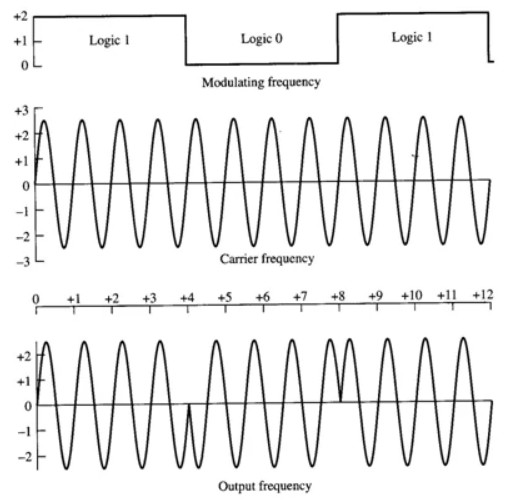
\includegraphics[width=0.8\textwidth]{figures/6-43.jpg}
    \caption{Dans ce modulateur, la porteuse prend l'une des deux phases. Un 1 logique ne produit aucun changement de phase et un 0 logique produit un changement de phase de 180°. Image par IDC Online.}
    \label{fig:communication2}
\end{figure}
\textbf{Modulation d'amplitude en quadrature (QAM) :}
\begin{itemize}
    \item La \textbf{modulation d'amplitude en quadrature} (\textbf{QAM}) permet de transmettre :
    \begin{itemize}
        \item Deux \textbf{signaux de message analogiques}, ou
        \item Deux \textbf{flux de bits numériques}.
    \end{itemize}
    \item La transmission est réalisée en \textbf{modulant les amplitudes} de deux ondes porteuses selon :
    \begin{itemize}
        \item Le schéma de \textbf{modulation numérique par déplacement d'amplitude} (ASK),
        \item Le schéma de \textbf{modulation analogique par modulation d'amplitude} (AM).
    \end{itemize}
    \item Ces deux ondes porteuses :
    \begin{itemize}
        \item Ont la \textbf{même fréquence},
        \item Sont \textbf{déphasées de 90°} (\textbf{quadrature} ou \textbf{orthogonalité}).
    \end{itemize}
    \item Le signal transmis est obtenu en \textbf{additionnant les deux ondes porteuses}.
    \item La QAM est applicable aux signaux :
    \begin{itemize}
        \item \textbf{Analogiques} (modulation d'amplitude analogique),
        \item \textbf{Numériques} (modulation numérique par ASK).
    \end{itemize}
\end{itemize}
\begin{figure}[H] % H force l'affichage ici
    \centering
    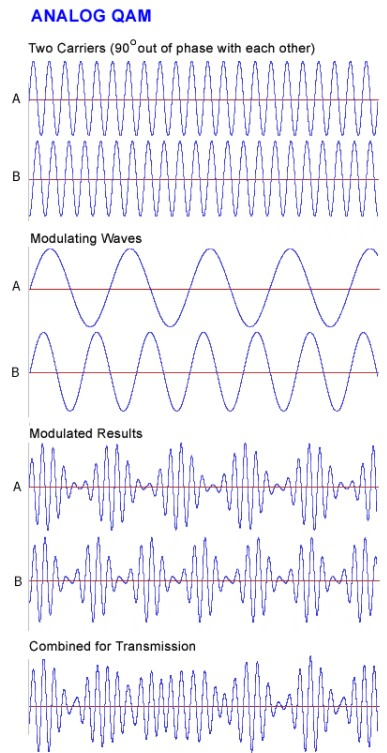
\includegraphics[width=0.8\textwidth]{figures/6-44.jpg}
    \caption{Démonstration étape par étape de la modulation QAM analogique à partir de deux ondes porteuses, d'ondes modulantes, d'ondes intermédiaires et du produit final. Image de The Free Dictionary.}
    \label{fig:communication2}
\end{figure}
\textbf{Modulation d'amplitude en quadrature (QAM) :}
\begin{itemize}
    \item Supposons un signal porteur sous la forme :
    \[
    c_1(t) = \cos(\omega_c t)
    \]
    \item Le décalage de phase de 90 degrés est donné par :
    \[
    c_2(t) = \cos(\omega_c t + \tfrac{\pi}{2})
    \]
    \item Dans un signal QAM :
    \begin{itemize}
        \item Une porteuse est en retard de 90° sur l'autre.
        \item La \textbf{modulation d'amplitude} de la première porteuse est appelée \textbf{composante en phase}, notée \( I(t) \).
        \item La modulation d'amplitude de la deuxième porteuse est appelée \textbf{composante en quadrature}, notée \( Q(t) \).
    \end{itemize}
    \item Ainsi, la forme d'onde composite du signal QAM est donnée par :
    \[
    s_{QAM}(t) = c_1(t) I(t) + c_2(t) Q(t)
    \]
\end{itemize}
\begin{figure}[H] % H force l'affichage ici
    \centering
    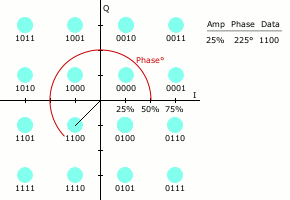
\includegraphics[width=0.8\textwidth]{figures/QAM16_Demonstration.png}
    \caption{Digital 16-QAM with example constellation points. Image by Chris Watts.}
    \label{fig:communication2}
\end{figure}
\textbf{Constellation et ordres de modulation en QAM :}
\begin{itemize}
    \item Comme pour de nombreux schémas de modulation numérique, le \textbf{diagramme de constellation} est utile pour la QAM.
    \item En QAM, les points de constellation sont généralement disposés en grille carrée avec un espacement vertical et horizontal égal.
    \item D'autres configurations sont possibles, telles que le \textbf{Cross-QAM}.
    \item Dans les télécommunications numériques, les données sont généralement binaires, donc le nombre de points dans la grille est souvent une puissance de 2 (2, 4, 8, ...).
    \item Les formes les plus courantes de QAM sont :
    \begin{itemize}
        \item \textbf{16-QAM}
        \item \textbf{64-QAM}
        \item \textbf{256-QAM}
    \end{itemize}
    \item En augmentant l'ordre de la constellation, il est possible de transmettre plus de bits par symbole.
    \item Toutefois, si l'énergie moyenne de la constellation reste constante :
    \begin{itemize}
        \item Les points doivent être plus rapprochés.
        \item Ils deviennent plus sensibles au bruit et aux autres interférences.
        \item Cela entraîne un \textbf{taux d'erreur binaire} (BER) plus élevé.
    \end{itemize}
    \item Une QAM d'ordre supérieur permet de transmettre plus de données mais avec une fiabilité moindre, à énergie de constellation moyenne constante.
    \item Pour utiliser une QAM d'ordre supérieur sans augmenter le taux d'erreur binaire, il est nécessaire d'améliorer le \textbf{rapport signal sur bruit} (SNR) en :
    \begin{itemize}
        \item Augmentant l'énergie du signal.
        \item Réduisant le bruit.
        \item Ou une combinaison des deux.
    \end{itemize}
\end{itemize}
Digital vs. Analog Modulation
In summary, analog and digital modulation modify an information signal with a carrier signal. The carrier signal is always a sinusoid at the licensed radiofrequency. The information signal can either be analog or digital, which defines the name of the modulation scheme.
The advantage of analog amplitude modulation conserves bandwidth and analog frequency modulation spreads information bandwidth over larger RF bandwidth. Digital pulse-code modulation (particularly phase-shift keying) uses RF power most efficiently.
\begin{figure}[H] % H force l'affichage ici
    \centering
    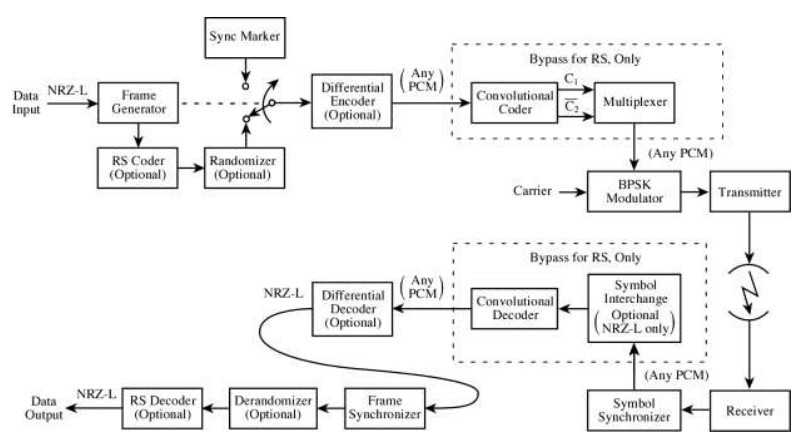
\includegraphics[width=0.8\textwidth]{figures/6-45.jpg}
    \caption{Spacecraft and Ground Configuration for BPSK Reed-Solomon, Convolutional, and Concatenated Coding Date, Andrew O’Dea, and Timothy T. Pham Date. “Telemetry Data Decoding.” (2013).}
    \label{fig:communication2}
\end{figure}
\textbf{Utilisation de la modulation en code binaire (PCM) dans les engins spatiaux :}
\begin{itemize}
    \item Tous les engins spatiaux modernes utilisent la \textbf{modulation par code binaire} (PCM) pour transférer des données binaires entre le vaisseau spatial et les opérations de mission.
    \item Les données sont modulées en phase sur une porteuse RF (\textbf{PCM/PM}) ou utilisées pour commuter la phase d'une sous-porteuse de plus ou moins \(\pm 90^\circ\).
    \item La sous-porteuse est ensuite modulée en phase sur la porteuse pour la transmission via le lien spatial.
    \item Ce schéma de modulation est appelé \textbf{PCM/PSK/PM} :
    \begin{itemize}
        \item \textbf{PCM} : Modulation par code binaire.
        \item \textbf{PSK} : Modulation par déplacement de phase de la sous-porteuse.
        \item \textbf{PM} : Modulation en phase sur la porteuse RF.
    \end{itemize}
    \item La modulation de phase est privilégiée car :
    \begin{itemize}
        \item Elle possède une \textbf{enveloppe constante}, permettant l'utilisation d'\textbf{amplificateurs non linéaires}.
        \item Les amplificateurs non linéaires sont généralement plus \textbf{efficaces} que les amplificateurs linéaires requis pour les modulations d'amplitude.
        \item Elle est \textbf{immunisée contre la plupart des interférences} affectant l'amplitude du signal.
    \end{itemize}
\end{itemize}
\textbf{Polarization}
\begin{figure}[H] % H force l'affichage ici
    \centering
    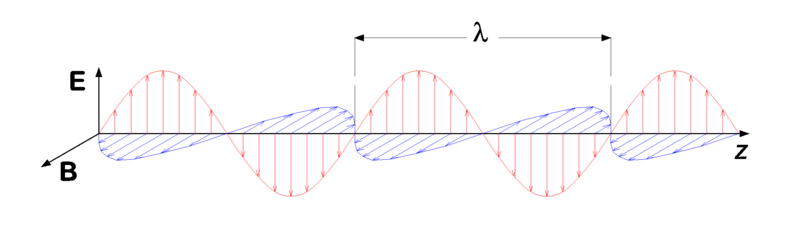
\includegraphics[width=0.8\textwidth]{figures/6-46.png}
    \caption{Polarization}
    \label{fig:communication2}
\end{figure}
Polarization refers to the orientation of the electric field vector, E. Waves can have different shapes: linear and circular. The shape is traced by the end of the vector at a fixed location, as observed along the direction of propagation.
\begin{figure}[H] % H force l'affichage ici
    \centering
    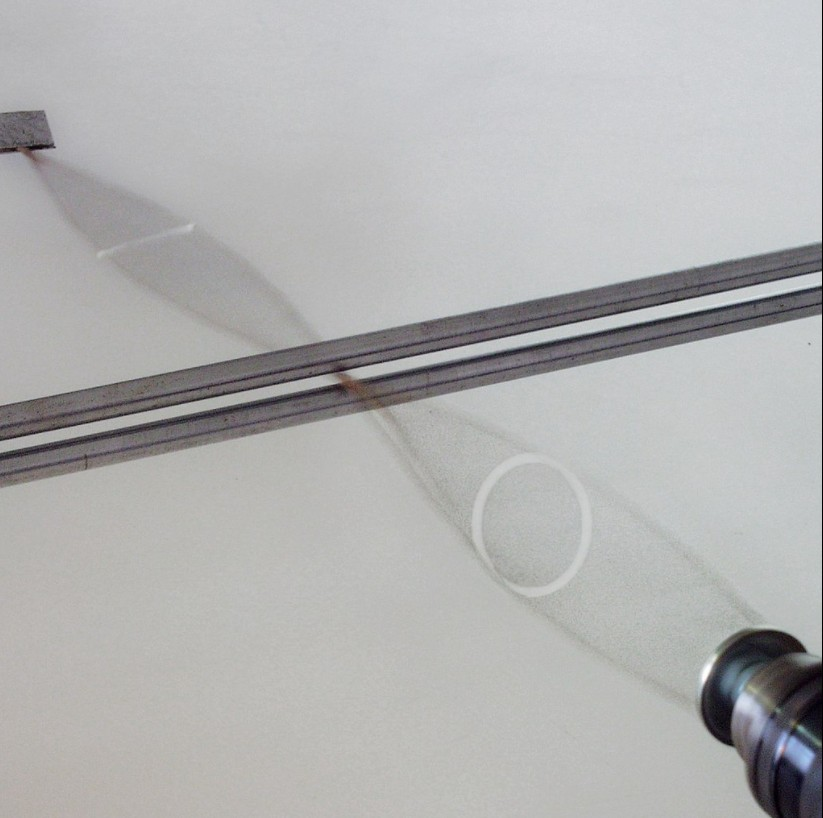
\includegraphics[width=0.8\textwidth]{figures/6-47.jpg}
    \caption{Circular polarization on rubber thread converted to linear polarization. CC BY-SA 3.0. Image by Zátonyi Sándor.}
    \label{fig:communication2}
\end{figure}
\textbf{Taux d'erreur binaire (Bit Error Rate - BER) :}
\begin{itemize}
    \item Le \textbf{BER} est la probabilité qu'une erreur soit commise sur un bit lors du décodage d'un symbole.
    \item C'est une mesure de la qualité des communications et l'une des exigences principales d'un système de communication.
    \item L'autre exigence majeure est le \textbf{débit de données} (quantité de données transmises).
    \item Exemple : Soit la séquence de bits transmise suivante :
    \begin{center}
        0 \quad 1 \quad 1 \quad 0 \quad 0 \quad 0 \quad 1 \quad 0 \quad 1 \quad 1
    \end{center}
    \item Et la séquence de bits reçue :
    \begin{center}
        0 \quad \underline{0} \quad 1 \quad 0 \quad \underline{1} \quad 0 \quad 1 \quad 0 \quad \underline{0} \quad 1
    \end{center}
    \item Le nombre d'erreurs est ici de \textbf{3} bits erronés.
    \item Le \textbf{BER} est donc : 
    \[
    \frac{3 \text{ bits incorrects}}{10 \text{ bits transmis}} = 0.3 \text{ (30\%)}
    \]
    \item Typiquement, le BER est de l'ordre de \(10^{-5}\).
    \item Des BER plus élevés peuvent être tolérés pour des applications non critiques.
\end{itemize}
\textbf{Le BER dépend de deux paramètres principaux :}
\begin{itemize}
    \item \textbf{Le rapport signal/bruit} (\textit{Signal-to-Noise Ratio - SNR}), généralement exprimé en fonction de :
    \[
    \frac{E_b}{N_0}
    \]
    où \(E_b\) est l'énergie par bit et \(N_0\) la densité spectrale de bruit.
    \item \textbf{La modulation utilisée} :
    \begin{itemize}
        \item Pour un même BER, \textbf{BPSK} et \textbf{QPSK} nécessitent \textbf{3 dB} de moins en \(\frac{E_b}{N_0}\) que \textbf{8PSK}.
    \end{itemize}
\end{itemize}
\textbf{Facteurs influençant le taux d'erreur binaire (BER) :}
\begin{itemize}
    \item Dans un système de communication, le BER côté récepteur peut être affecté par :
    \begin{itemize}
        \item \textbf{Le bruit du canal de transmission}.
        \item \textbf{Les interférences et la distorsion}.
        \item \textbf{Les problèmes de synchronisation des bits}.
        \item \textbf{L'atténuation du signal}.
        \item \textbf{L'évanouissement multipath en transmission sans fil}.
    \end{itemize}
    \item Le BER peut être amélioré par :
    \begin{itemize}
        \item \textbf{Le choix d'une puissance de signal plus élevée}, à condition d'éviter la diaphonie (\textit{cross-talk}) qui peut augmenter les erreurs de bits.
        \item \textbf{L'utilisation d'un schéma de modulation lent et robuste}.
        \item \textbf{L'application de schémas de codage de ligne optimisés}.
        \item \textbf{L'implémentation de codes correcteurs d'erreur} (\textit{Forward Error Correction - FEC}).
    \end{itemize}
\end{itemize}
\textbf{Types de BER :}
\begin{itemize}
    \item \textbf{Le BER de transmission} est défini comme :
    \[
    \frac{\text{Nombre de bits erronés détectés avant correction}}{\text{Nombre total de bits transmis (y compris les codes d'erreur redondants)}}
    \]
    \item \textbf{Le BER d'information} est approximativement égal à la probabilité d'erreur après décodage :
    \[
    \frac{\text{Nombre de bits incorrects après correction}}{\text{Nombre total de bits décodés (information utile)}}
    \]
    \item En général :
    \[
    \text{BER de transmission} > \text{BER d'information}
    \]
    \item Le BER d'information est influencé par la robustesse du \textbf{code correcteur d'erreur} utilisé.
\end{itemize}
\begin{figure}[H] % H force l'affichage ici
    \centering
    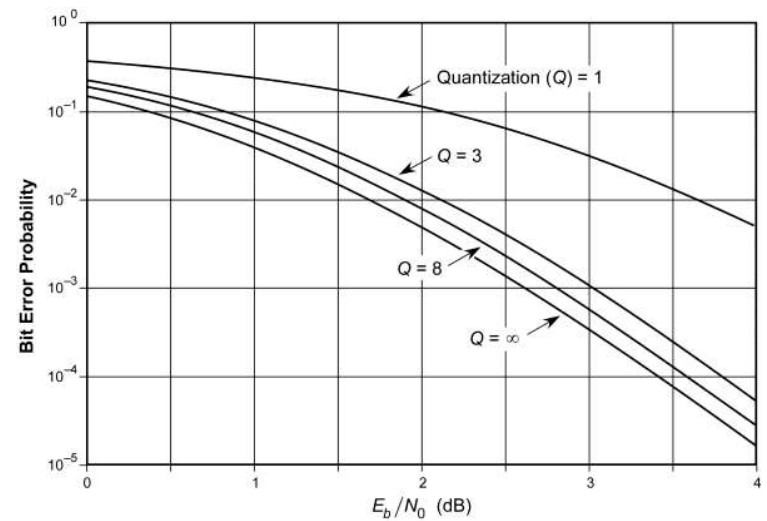
\includegraphics[width=0.8\textwidth]{figures/6-48.jpg}
    \caption{Quantization Effects on Decoder Performance. Date, Andrew O’Dea, and Timothy T. Pham Date. “Telemetry Data Decoding.” (2013).}
    \label{fig:communication2}
\end{figure}
\textbf{Calcul du BER en fonction du rapport signal sur bruit énergétique $\frac{E_b}{N_0}$ pour la modulation BPSK :}
Nous considérons un signal BPSK avec une porteuse où $t$ est le temps et $T$ est la période. Le signal d'information est donné par :
\[
x_1 (t) = + A \sqcap\left(\frac{t}{T} \right), \quad x_0 (t) = - A \sqcap\left(\frac{t}{T} \right)
\]
où $\sqcap(t)$ est une fonction porte.
\textbf{Effet du canal de transmission :}
Le canal (c'est-à-dire l’atmosphère et l’électronique du récepteur) ajoute un bruit blanc gaussien $n(t)$ de moyenne nulle et de variance :
\[
\sigma^2 = \frac{N_0}{2} B = \frac{N_0}{2T}
\]
\textbf{Distribution du signal reçu :}
La probabilité de réception du signal est alors une distribution gaussienne centrée autour de $+A$ ou $-A$ selon le symbole transmis.
\begin{figure}[H] % H force l'affichage ici
    \centering
    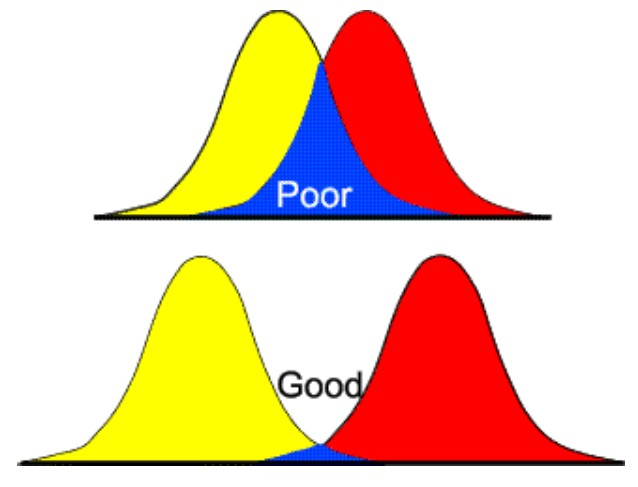
\includegraphics[width=0.8\textwidth]{figures/6-49.jpg}
    \caption{The probability distribution of getting the bit that was intended in a transmission. Gaussians around + 1 and – 1. If the variance is large enough, these probability distributions overlap (blue region). A symbol in that region would be ambiguous. Image by Alan Fielding.}
    \label{fig:communication2}
\end{figure}
\textbf{Calcul du BER en modulation BPSK :}
Les deux distributions de probabilité se chevauchent. Si elles ne se chevauchaient pas, il serait possible d’établir une règle de décision parfaite qui permettrait toujours d’identifier correctement le symbole transmis en fonction de la tension reçue. Cela pourrait être le cas pour un bruit de variance plus faible ou de forme différente, comme un bruit triangulaire avec une bande passante inférieure à $A$.
La meilleure règle imparfaite qui minimise la probabilité d'erreur est la règle du \textbf{Maximum A Posteriori} (MAP). Intuitivement, dans ce cas simple, nous décidons qu'un \textbf{1} a été envoyé si la tension reçue est positive, et qu’un \textbf{0} a été envoyé si elle est négative. De manière générale, il s'agit d'un problème de classification bien connu (ou de test d'hypothèses) dont la solution est établie.
\textbf{Calcul du BER :}
La probabilité d’erreur résiduelle (\textit{Bit Error Rate}, BER) est donnée par :
\begin{align*} 
BER &= P(\text{envoyer } 0) \cdot P(\text{décider } 1 | \text{envoyé } 0 ) + P(\text{envoyer } 1) \cdot P(\text{décider } 0 | \text{envoyé } 1) \\ 
&= 0.5 P(1|0) + 0.5 P(0|1) \\ 
&= 0.5 P (N( - A,\sigma^2)>0) + 0.5 P (N( + A,\sigma^2)<0) \\ 
&= P (N( + A,\sigma^2)<0) \\ 
&= \frac{1}{\sqrt{2\pi} \sigma} \int_0^\infty e^{-\frac{1}{2} \left(\frac{x+A}{\sigma}\right)^2} dx \\ 
&= \frac{1}{\sqrt{2\pi}} \int_{\frac{A}{\sigma}}^\infty e^{-\frac{1}{2} t^2} dt \\ 
&\equiv Q \left( \frac{A}{\sigma} \right)
\end{align*}
\textbf{Expression en fonction du rapport signal sur bruit énergétique :}
Le \textit{Bit Error Rate} (BER) est généralement exprimé en fonction du rapport $\frac{E_b}{N_0}$ :
\[BER = Q \left(\frac{A}{\sigma} \right)\]
Le BER peut être calculé pour d'autres modulations en utilisant une approche similaire. Par exemple :
\[BER_{QPSK} \approx Q \left( \sqrt{2 \frac{E_b}{N_0}} \right)\]
\[BER_{8PSK} \approx \frac{2}{3} Q \left( \sqrt{2 \frac{E_b}{N_0}} \sin \frac{\pi}{8} \right)S\]
\begin{figure}[H] % H force l'affichage ici
    \centering
    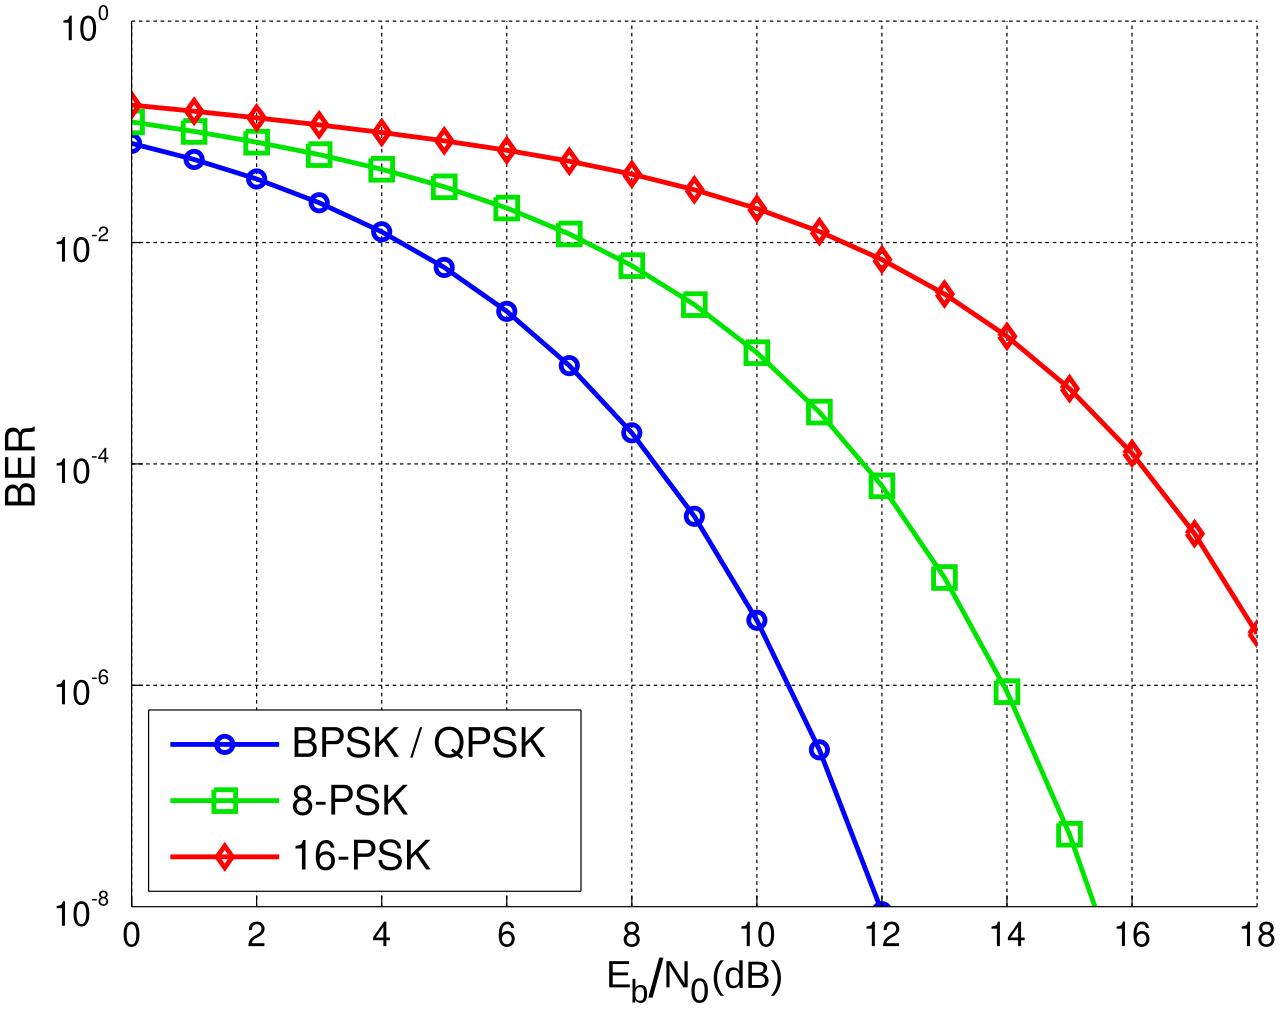
\includegraphics[width=0.8\textwidth]{figures/6-50.png}
    \caption{Bit-error rate (BER) vs Eb/N0 curves for different digital modulation methods is a common application example of Eb/N0. Here an AWGN channel is assumed. CC BY-SA 3.0. Image by Splash.}
    \label{fig:communication2}
\end{figure}
\textbf{Effet des codes correcteurs d'erreurs sur le BER :}
L'ajout de schémas de codage tels que \textbf{Reed-Solomon} ou \textbf{Viterbi} à une modulation permet d'améliorer la robustesse du système face au bruit et aux interférences. En pratique, ces codes correcteurs d'erreurs ont pour effet de \textbf{déplacer la courbe} $BER = f(\tfrac{E_b}{N_0})$ vers la gauche. Cela signifie qu'une puissance \textbf{inférieure} est requise pour atteindre un certain taux d'erreur binaire donné.
\textbf{Effet des codes sur la performance du système :}
\begin{itemize}
    \item \textbf{Codage de convolution (Viterbi)} : Utilisé pour détecter et corriger les erreurs sur des canaux affectés par un bruit gaussien blanc additif (AWGN) ou par des interférences. L'algorithme de Viterbi maximise la vraisemblance du message reçu.
    \item \textbf{Codes Reed-Solomon} : Particulièrement efficaces pour corriger les erreurs en rafale, ils sont souvent utilisés en conjonction avec un codage convolutif dans un schéma dit de \textbf{codage en cascade}.
\end{itemize}
L'effet global du codage d'erreur est de réduire la probabilité d'erreur binaire $BER$ pour un même rapport signal-sur-bruit énergétique $\tfrac{E_b}{N_0}$. Ce gain est souvent mesuré en \textbf{gain de codage}, défini comme la réduction en dB de $\tfrac{E_b}{N_0}$ nécessaire pour obtenir un BER donné.
